%%% TESTs


% The role of the architect

%1
\newcommand{\qPragmaticArchitect}{
\begin{ClosedQuestion}
	According to Frank Buschmann in the article \emph{Introducing the Pragmatic Architect}
		
    \optionA{The business aspects of the system are for business architects, not the software architects.}
    \optionB{Dealing with the technological aspects of the system should be delayed to the implementation stage of development.}
    \optionC{The modeling of a system is not part of the software architect duties.}
    \optionD{The level of abstraction of the system an architect works may vary.}
 \putOptions 
\end{ClosedQuestion}
}

%2
\newcommand{\qArchitecturalInfluenceCycle}{
\begin{ClosedQuestion}
	Suppose that after designing a successful architecture for a particular client the software house management decides to create a cross-functional internal department to start providing products for this particular segment of the market.
		
    \optionA{This is a case of an architectural influence cycle where the feedback cycle resulted in changes on the business.}
    \optionB{This is a case of an architectural influence cycle where the feedback cycle resulted in changes on the project.}
    \optionC{This is a case of an architectural influence cycle where the feedback cycle resulted in changes on the business and project.}
    \optionD{This is a case of an architectural influence cycle without feedback.}
 \putOptions 
\end{ClosedQuestion}
}

%3
\newcommand{\qDiplomat}{
\begin{ClosedQuestion}
	Very often, when a software architecture is being designed, conflicting requirements are identified, like between security and availability. The role of the software architect is to
		
    \optionA{Design an architectural solution together with the stakeholders to be sure that everybody agrees on the resolution of conflits.}
    \optionB{Solve the conflicts between requirements by deciding on the best trad-offs the system should support.}
    \optionC{Facilitate the communication among the stakeholders such that they can decide on what are the architecturally significant requirements.}
    \optionD{Design an architecture that supports all the conflicting requirements and present it to the stakeholders.}
 \putOptions 
\end{ClosedQuestion}
}

\newcommand{\qDiplomatPT}{
\begin{ClosedQuestion}
	Frequentemente, quando uma arquitetura de software é desenhada, são identificados requisitos conflituosos, como seja entre segurança e disponibilidade. O papel da arquitetura de software é
		
    \optionA{Desenhar uma solução arquitetural conjuntamente com os \emph{stakeholders} para ter a certeza que todas as partes concordam com a resolução de conflitos.}
    \optionB{Resolver os conflitos entre os requisitos decidindo quais os compromissos que o sistema deve suportar.}
    \optionC{Facilitar a comunicação entre os \emph{stakeholders} de forma a que eles decidam quais são os requisitos arquiteturalmente relevantes.}
    \optionD{Desenhar uma arquitetura que suporta todos os requisitos conflituosos e apresentá-la aos \emph{stakeholders}.}
 \putOptions 
\end{ClosedQuestion}
}

% The Software Architecture

%4
\newcommand{\qEarlydDecisions}{
\begin{ClosedQuestion}
	In his article \emph{Who Needs an Architect?} Martin Fowler refers to the following architecture definition
		
	\begin{quote}
		\emph{architecture is the set of design decisions that must be made early in a project}
	\end{quote}

    \optionA{Martin Fowler disagrees with this definition because we should delay the design decisions and focus on features first.}
    \optionB{Martin Fowler complains about this definition because the early decisions are not necessarily the right ones.}
    \optionC{Martin Fowler complains about this definition because architecture should stress flexibility which can only be necessary later.}
    \optionD{Martin Fowler disagrees with this definition because to design an architecture it is not necessary to make any decision.}
 \putOptions 
\end{ClosedQuestion}
}

%5
\newcommand{\qSharedUnderstanding}{
\begin{ClosedQuestion}
	In his article \emph{Who Needs an Architect?} Martin Fowler refers to the following architecture definition
		
	\begin{quote}
		\emph{the expert developers working on that project have a shared understanding of the system design}
	\end{quote}

    \optionA{This shared understanding can be represented by a set of architectural views.}
    \optionB{This shared understanding includes the architecturally significant requirements.}
    \optionC{The system algorithms should be part of the shared understanding.}
    \optionD{The shared understanding describes the system from a high-level perspective.}
 \putOptions 
\end{ClosedQuestion}
}

%6
\newcommand{\qASDefinition}{
\begin{ClosedQuestion}
	The definition of software architecture, on the course book, is
	\begin{quote}
		\emph{The software architecture of a system is the set of structures needed to reason about the system, which comprise software elements, relations among them, and properties of both.}
	\end{quote}
	
	According to this definition

    \optionA{The set of structures is needed to support different levels of performance for the system.}
    \optionB{To reason about a system is to verify whether the architecturally significant requirements are considered by the architecture.}
    \optionC{The hardware is an example of a software element.}
    \optionD{There isn't any relation between the properties of the software elements and the ability to reason about the system.}
 \putOptions 
\end{ClosedQuestion}
}

\newcommand{\qASDefinitionPT}{
\begin{ClosedQuestion}
	A definição da arquitetura de software no livro é
	\begin{quote}
		\emph{The software architecture of a system is the set of structures needed to reason about the system, which comprise software elements, relations among them, and properties of both.}
	\end{quote}
	
	De acordo com esta definição

    \optionA{Um conjunto de estruturas é necessário para suportar os diferentes níveis de desempenho do sistema.}
    \optionB{Raciocinar acerca do sistema é verificar se os requisitos arquiteturalmente relevantes são considerados pela arquitetura.}
    \optionC{O hardware é um exemplo de um elemento de software.}
    \optionD{Não existe nenhuma relação entre as propriedades dos elementos de software e a capacidade de raciocinar acerca do sistema.}
 \putOptions 
\end{ClosedQuestion}
}

% Architectures for scalable web applications

%7
\newcommand{\qImageHostingPerformance}{
\begin{ClosedQuestion}
	Consider the following informal view of an Image Hosting System
	
\begin{center}
	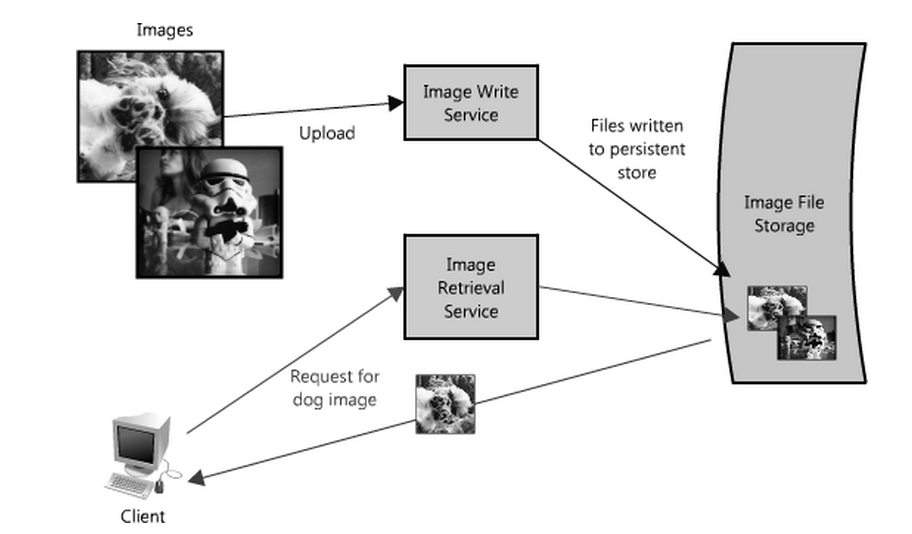
\includegraphics[width=100mm]{ImageHostingPerformance}
\end{center}

    \optionA{This view highlights the availability of the system.}
    \optionB{This view highlights the performance of the \texttt{Image File Storage}.}
    \optionC{This view highlights the different performance levels for \texttt{upload} and \texttt{dowload} operations.}
    \optionD{This view highlights the scalability of \texttt{upload} and \texttt{dowload} operations.}
 \putOptions 
\end{ClosedQuestion}
}

%8
\newcommand{\qImageHostingScalability}{
\begin{ClosedQuestion}
	Consider the following informal view of an Image Hosting System
	
\begin{center}
	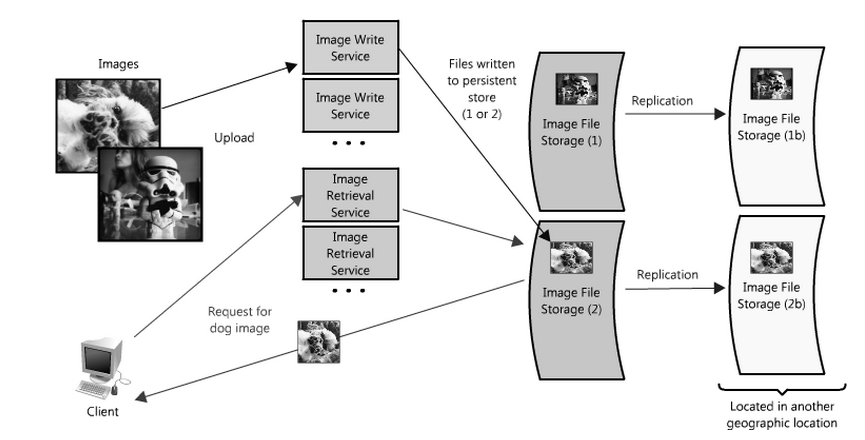
\includegraphics[width=100mm]{ImageHostingScalability}
\end{center}

    \optionA{This view highlights the security of the system.}
    \optionB{This view highlights the scalability of \texttt{upload} and \texttt{dowload} operations.}
    \optionC{This view highlights the scalability of storage.}
    \optionD{This view highlights the scalability of \texttt{upload} and \texttt{dowload} operations, and of storage.}
 \putOptions 
\end{ClosedQuestion}
}

%9
\newcommand{\qImageHostingReads}{
\begin{ClosedQuestion}
	Consider the following informal view of an Image Hosting System
	
\begin{center}
	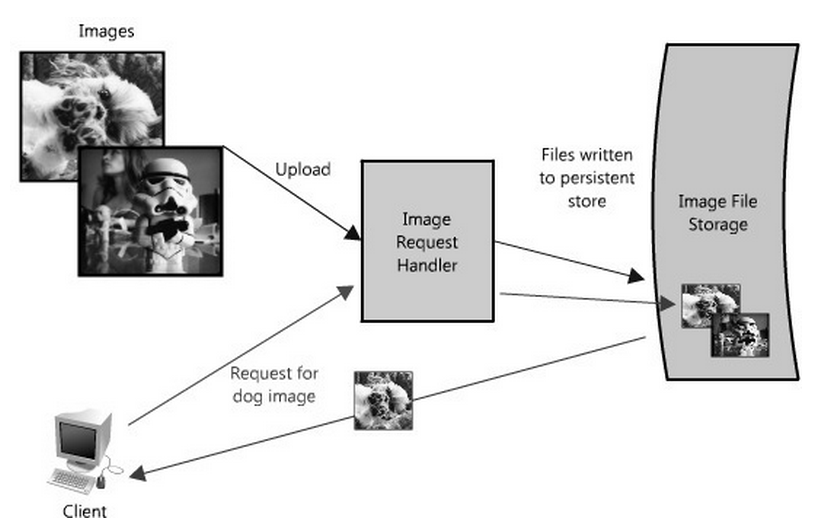
\includegraphics[width=100mm]{ImageHostingReads}
\end{center}

    \optionA{This view highlights the availability of the \texttt{Image File Storage}.}
    \optionB{This view highlights the performance of the \texttt{download} operations.}
    \optionC{This view highlights the performance of \texttt{upload} operations.}
    \optionD{This view highlights the scalability of \texttt{upload} and \texttt{dowload} operations.}
 \putOptions 
\end{ClosedQuestion}
}

\newcommand{\qImageHostingReadsPT}{
\begin{ClosedQuestion}
	Considere a seguinte vista informal de um Image Hosting System
	
\begin{center}
	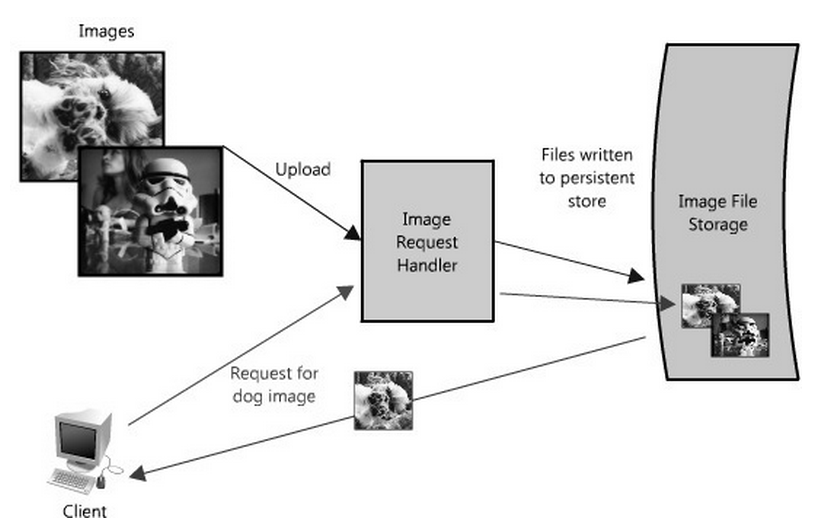
\includegraphics[width=100mm]{ImageHostingReads}
\end{center}

    \optionA{Esta vista dá relevância à disponibilidade do \texttt{Image File Storage}.}
    \optionB{Esta vista dá relevância ao desempenho das operações de \texttt{download}.}
    \optionC{Esta vista dá relevância ao desempenho das operações de \texttt{upload}.}
    \optionD{Esta vista dá relevância à escalabilidade das operações de \texttt{upload} e \texttt{dowload}.}
 \putOptions 
\end{ClosedQuestion}
}

% Requirements

%10
\newcommand{\qGeneralScenario}{
\begin{ClosedQuestion}
	A general scenario for a quality attribute

    \optionA{Should be avoided because scenarios should describe very concrete situations.}
    \optionB{Enumerates, for each kind of quality attribute, all the possible types of source of stimulus, stimulus, etc.}
    \optionC{Can omit some of the elements like, for instance, the environment, if they are not relevant for the general scenario.}
    \optionD{Is a very reusable scenario that can be used in many different concrete situations.}
 \putOptions 
\end{ClosedQuestion}
}

%11
\newcommand{\qInteroperabilityStimulus}{
\begin{ClosedQuestion}
	In a scenario for interoperability

    \optionA{The exchange of information is the stimulus.}
    \optionB{The request to adapt an interface is the stimulus.}
    \optionC{The design of a reusable interface is the stimulus.}
    \optionD{The data input to the system is the stimulus.}
 \putOptions 
\end{ClosedQuestion}
}

%12
\newcommand{\qRequirementsImpact}{
\begin{ClosedQuestion}
	The requirements impact on how an architecture is designed

    \optionA{However, functional requirements do not have any impact on the architecture because the systemic qualities of an architecture are non-functional.}
    \optionB{The functional requirements have a large impact on the definition of views of the component-and-connector viewtype because each component executes a functionality.}
    \optionC{The functional requirements have a large impact on the definition of views of the module viewtype because they are used to define the high cohesion and low coupling of modules.}
    \optionD{The functional requirements can be considered as constraints on the software architecture design.}
 \putOptions 
\end{ClosedQuestion}
}

\newcommand{\qRequirementsImpactPT}{
\begin{ClosedQuestion}
	Os requisitos têm um impacto sobre como a arquitetura é desenhada

    \optionA{Contudo, os requisitos funcionais não têm nenhum impacto na arquitetura pois as qualidades sistémicas de uma arquitetura são não funcionais.}
    \optionB{Os requisitos funcionais têm um grande impacto na definição tipo vista componente-e-conetor porque cada componente executa uma funcionalidade.}
    \optionC{Os requisitos funcionais têm uma grande impactos na definição de vistas do tipo vista módulo porque elas são usadas para definir a coesão forte e a ligação fraca.}
    \optionD{Os requisitos funcionais podem ser considerados como as restrições sobre o desenho da arquitetura de software.}
 \putOptions 
\end{ClosedQuestion}
}

% Availability scenarios and tactics

%13
\newcommand{\qOmissionRetry}{
\begin{ClosedQuestion}
	Considering the availability architectural quality, the tactic of retry

    \optionA{Can be applied to any kind of availability scenario.}
    \optionB{Is useful to support scenarios where the stimulus is an omission.}
    \optionC{Guarantees that the system will not become unavailable.}
    \optionD{Reduces the availability scenario response time because the request occurs twice.}
 \putOptions 
\end{ClosedQuestion}
}

%14
\newcommand{\qPingEchoHeartbeat}{
\begin{ClosedQuestion}
	Considering the availability architectural quality and the tactics of ping/echo and heartbeat

    \optionA{These tactics cannot not be applied in conjunction with the self-test tactic.}
    \optionB{These tactics are used to prevent the occurence of a fault.}
    \optionC{Heartbeat is more scalable than ping/echo because the monitor does not need to know in advance the addresses of the components.}
    \optionD{In ping/echo the components have the initiative to start the interaction.}
 \putOptions 
\end{ClosedQuestion}
}

%15
\newcommand{\qRestartInRedundancy}{
\begin{ClosedQuestion}
	Considering the availability architectural quality and the tactics of active redundancy, passive redundancy, and spare

    \optionA{Active redundancy can be used together with a voting tactic to detect and recover from faults.}
    \optionB{These tactics are used to prevent the occurence of a fault.}
    \optionC{Spare guarantees immediate recover.}
    \optionD{Passive redundancy does not work with non-deterministic behavior of request's execution.}
 \putOptions 
\end{ClosedQuestion}
}

\newcommand{\qRestartInRedundancyPT}{
\begin{ClosedQuestion}
	Considerando a qualidade arquitetural da disponibilidade e as táticas de redundância ativa, redundância passiva e substituição

    \optionA{A redundância ativa pode ser usada conjuntamente com uma tática de votação para detectar e recuperar de faltas.}
    \optionB{Estas táticas são usadas para prevenir a ocorrência de faltas.}
    \optionC{Substituição garante recuperação imediata.}
    \optionD{Redundância passiva não funciona com comportamento não determinista durante a execução.}
 \putOptions 
\end{ClosedQuestion}
}


%1
\newcommand{\qFeaturitis}{
\begin{ClosedQuestion}
	Frank Buschmann states that:
		
	\begin{quote}
		Featuritis is the tendency to trade functional coverage for quality - the more functions the earlier they're delivered, the better.
	\end{quote}

    \optionA{Featuritis may result from a requirement of the technical context.}
    \optionB{Featuritis requires the performance quality because the end user needs to execute the features.}
    \optionC{Featuritis may be a result of a requirement of the business context.}
    \optionD{Featuritis requires the modifiability quality to allow a the system to be easily modified to support new features.}
 \putOptions 
\end{ClosedQuestion}
}

%2
\newcommand{\qExplicit}{
\begin{ClosedQuestion}
	Frank Buschmann states that:
	
	\begin{quote}
		There's only one escape from such situations: architects must actively break the cycle of mutual misunderstanding and mistrust!
	\end{quote}

    \optionA{Such misunderstanding and mistrust occurs because the stakeholders have their own agendas}
    \optionB{The cycle Frank Buschmann refers to is the Architectural Influence Cycle.}
    \optionC{The cycle Frank Buschmann refers to allows the clarification of requirements.}
    \optionD{To break such misunderstanding and mistrust the architecture has to make explicit the stakeholders needs.}
 \putOptions
\end{ClosedQuestion}
}

%3
\newcommand{\qFlexibilitis}{
\begin{ClosedQuestion}
	Frank Buschmann states that:
	
	\begin{quote}
		Overly flexible systems are hard to configure, and when they're finally configured, they lack qualities like performance or security.
	\end{quote}

    \optionA{Frank Buschmann is referring to some possible consequences of the modifiability quality.}
    \optionB{Frank Buschmann are considering performance and security as the most important qualities.}
    \optionC{Frank Buschmann is referring that the consequences of a flexible system is poor performance and bad security.}
    \optionD{Frank Buschmann is not considering modifiability as an important quality}
 \putOptions
\end{ClosedQuestion}
}

%4
\newcommand{\qPrioritize}{
\begin{ClosedQuestion}
	Frank Buschmann states that:
	
	\begin{quote}
		Architects use flexibility as a cover for uncertainty.
	\end{quote}

    \optionA{A flexible architecture occurs when it is not possible to identify all the requirements.}
    \optionB{A solution to this problem is to prioritize the system qualities.}
    \optionC{Performance uncertainty about the system should be dealt with more flexibility.}
    \optionD{A solution to this problem is to reduce the level of flexibility of a system.}
 \putOptions
\end{ClosedQuestion}
}

%5
\newcommand{\qPerformitis}{
\begin{ClosedQuestion}
	Frank Buschmann cites the characterization Marquardt does of Performitis:
		
	\begin{quote}
		Each part of the system is directly influenced by local performance tuning measures. There is no global performance strategy, or it ignores other qualities of the system as testability and maintainability.
	\end{quote}
	
	From this problem you can conclude that:

    \optionA{Performance is a quality that you have to address at the end of the development process.}
    \optionB{There is no system which can have good performance and be easily maintainable.}
    \optionC{We have to distinguish architectural performance from opportunistic performance.}
    \optionD{The system performance quality has impact on the performance of the execution of tests.}
 \putOptions
\end{ClosedQuestion}
}

%6
\newcommand{\qFeaturitisPerformitisFlexibilities}{
\begin{ClosedQuestion}
	In his article, \emph{Featuritis, Performitis, and Other Deseases}, Frank Buschmann claims that:

    \optionA{Performance should be the last quality to be addressed because it is a local property of an architecture.}
    \optionB{Modifiability, flexibility, should be the first quality to be addressed because it allows the delay of architectural decisions.}
    \optionC{The lack of functionality results in a system without business value, therefore a rich set of features should be implemented first.}
    \optionD{A solution for any quality in isolation may lead to a biased architecture.}
 \putOptions
\end{ClosedQuestion}
}

%7
\newcommand{\qWalkingSkeleton}{
\begin{ClosedQuestion}
	The \emph{Walking Skeleton} referred in Frank Buschmann's article, \emph{Featuritis, Performitis, and Other Deseases}:

    \optionA{Is a functional prototype, which tests the functionalities required by the business stakeholders.}
    \optionB{Is an architecture that demonstrates that the system will support the qualities raised by the stakeholders.}
    \optionC{Is a baseline architecture that allows to experiment with the most significant architectural requirements.}
    \optionD{Is an object-oriented framework, which integrates functional and non-functional requirements of the system.}
 \putOptions
\end{ClosedQuestion}
}

%8
\newcommand{\qHammersNails}{
\begin{ClosedQuestion}
	In his article \emph{On Hammers and Nails, and Falling in Love with Technology and Design} what is the main type of influence on the architecture?

    \optionA{Project and Technical Contexts.}
    \optionB{Project and Professional Contexts.}
    \optionC{Business and Project Contexts.}
    \optionD{Professional and Technical Contexts.}
 \putOptions
\end{ClosedQuestion}
}

%9
\newcommand{\qArchitectureDefinition}{
\begin{ClosedQuestion}
	On the course slides you can find the following definition of architecture:
	
	\begin{quote}
		The software architecture of a program or computing system is the structure or structures of the system, which comprise software elements, the externally visible properties of those elements, and the relationships among them.
	\end{quote}
	
	However, in the book you can find another definition:
	
	\begin{quote}
		The software architecture of a system is the set of structures needed to reason about the system, which comprise the software elements, relations among them, and the properties of both.
	\end{quote}

    \optionA{The book definition does not consider relevant the externally visible properties.}
    \optionB{The book definition also considers that the properties are externally visible because they are used for reasoning by the stakeholders.}
    \optionC{The book definition also considers that the properties are externally visible because by definition an architectural property is externally visible.}
    \optionD{The book definition is not correct, as pointed out in the errata.}
 \putOptions
\end{ClosedQuestion}
}

%10
\newcommand{\qComponentvsModule}{
\begin{ClosedQuestion}
	In wikipedia you can find the following fragment of a definition:
	
	\begin{quote}
		An individual software component is a software package, or a module that encapsulates a set of related functions.
	\end{quote}
	
	According to the definitions taught in the course the above \emph{individual software component} corresponds to:

    \optionA{A component.}
    \optionB{A module.}
    \optionC{Both, a component and a module, depending on the perspective.}
    \optionD{An external element.}
 \putOptions
\end{ClosedQuestion}
}

%11
\newcommand{\qComponentvsModuleTwo}{
\begin{ClosedQuestion}
	In the Java documentation you can find:
	
\begin{quote}
\texttt{public abstract class Component} \\*
\texttt{extends Object} \\*
\texttt{implements ImageObserver, MenuContainer, Serializable}
\end{quote}

	Class \texttt{Component} is:

    \optionA{A component.}
    \optionB{A module.}
    \optionC{Both, a component and a module, depending on the perspective.}
    \optionD{An external element.}
 \putOptions
\end{ClosedQuestion}
}

%12
\newcommand{\qFunctionalModule}{
\begin{ClosedQuestion}
	When designing an architecture requirements can be split into functional, quality attributes, and constraints. Functional requirements have impact on:
		
    \optionA{A module view.}
    \optionB{A component-and-connector view.}
    \optionC{An allocation view.}
    \optionD{They are not represented by a view.}
 \putOptions
\end{ClosedQuestion}
}

%13
\newcommand{\qModuleViewType}{
\begin{ClosedQuestion}
	The quality that is more relevant to views of the module viewtype is:
		
    \optionA{Modifiability.}
    \optionB{Usability.}
    \optionC{Security.}
    \optionD{Availability.}
 \putOptions
\end{ClosedQuestion}
}

%14
\newcommand{\qComponentViewType}{
\begin{ClosedQuestion}
	The quality(ies) that is(are) more relevant to views of the component-and-connector viewtype is(are):
		
    \optionA{Modifiability.}
    \optionB{Availability and Performance.}
    \optionC{Testability.}
    \optionD{Availability.}
 \putOptions
\end{ClosedQuestion}
}

%15
\newcommand{\qEarlyDecisions}{
\begin{ClosedQuestion}
	In his article, \emph{Who Needs and Architect?}, Martin Fowler cites Ralph Johnson definition:
	
	\begin{quote}
		Architecture is the set of decisions that must be made early in a project.
	\end{quote}
	
	In his opinion:
		
    \optionA{This is right because if you don't the project fails.}
    \optionB{This is wrong because you can easily change these decisions during the project lifetime.}
    \optionC{This is right but you cannot be completely sure whether the decisions are the right ones.}
    \optionD{This is wrong because it is against agile way of thinking the software development process.}
 \putOptions
\end{ClosedQuestion}
}

%16
\newcommand{\qSharedUnderstandingTwo}{
\begin{ClosedQuestion}
	Martin Fowler, \emph{Who Needs and Architect?}, cites Ralph Johnson sentence:
	
	\begin{quote}
		In most successful software projects, the expert developers working on that project have a shared understanding of the system design. This shared understanding is called architecture.
	\end{quote}
			
    \optionA{This shared understanding is what distinguishes architecture from design.}
    \optionB{This shared understanding is necessary to define precise requirements.}
    \optionC{This shared understanding does not allow to define the architecture trade-offs because some of the stakeholders have their own goals.}
    \optionD{This shared understanding does not allow to have a global perspective of the system, because stakeholders have different interests.}
 \putOptions
\end{ClosedQuestion}
}

%17
\newcommand{\qArchitectDwarves}{
\begin{ClosedQuestion}
	Frank Buschmann, \emph{Introducing the Pragmatic Architect}, defines the \emph{architecture dwarves}. These kind of architects
	
    \optionA{Are unable to understand the technology capabilities.}
    \optionB{Are focused on the project context of the architecture.}
    \optionC{Are unable to distinguish architecture from design.}
    \optionD{Are focused on the business context of the architecture.}
 \putOptions
\end{ClosedQuestion}
}

%18
\newcommand{\qArchitectAstronauts}{
\begin{ClosedQuestion}
	Frank Buschmann, \emph{Introducing the Pragmatic Architect}, defines the \emph{architecture astronauts}. This kind of architect
	
    \optionA{Is unable to define a domain model of the system.}
    \optionB{Is focused on the technology context of the architecture.}
    \optionC{Is focused on creating common generalizations of several systems.}
    \optionD{Is focused on the details of the architecture.}
 \putOptions
\end{ClosedQuestion}
}

%19
\newcommand{\qCreateArchitectureOne}{
\begin{ClosedQuestion}
	During the different steps on how to create an architecture, the precise specification of architecture quality attributes is initially relevant to
	
    \optionA{Make a business case for the system.}
    \optionB{Understand the architecturally significant requirements.}
    \optionC{The system design.}
    \optionD{Documenting and communicating the architecture.}
 \putOptions
\end{ClosedQuestion}
}

%20
\newcommand{\qCreateArchitectureTwo}{
\begin{ClosedQuestion}
	The \emph{Ensuring that the implementation conforms to the architecture} step of how to create an architecture
	
    \optionA{Tries to guarantee that the final system will have the qualities required by stakeholders.}
    \optionB{Tries to guarantee that the final system will have the qualities aimed by the architecture.}
    \optionC{Does not allow developers to define some of the design of the system}
    \optionD{It requires automatic generation of code from the architecture.}
 \putOptions
\end{ClosedQuestion}
}





% Scenarios and Tactics

%1
\newcommand{\qAvailabilityScenario}{
\begin{ClosedQuestion}
	Consider the following scenario
	
	\begin{quote}
		When writing to the database the system receives an exception about a write failure. The system should stop interacting with data base and write a log message. 
	\end{quote}
	
	The quality addressed by this scenario is

    \optionA{Performance.}
    \optionB{Availability.}
    \optionC{Reliability.}
    \optionD{Fault-tolerance}
 \putOptions
\end{ClosedQuestion}
}

%2
\newcommand{\qScenario}{
\begin{ClosedQuestion}
	In a quality scenario

    \optionA{The stimulus is a system input.}
    \optionB{The response can be omitted.}
    \optionC{The artefact can be outside the system.}
    \optionD{The stimulus and the response should be always present.}
 \putOptions
\end{ClosedQuestion}
}


%3
\newcommand{\qTactics}{
\begin{ClosedQuestion}
	An architectural tactic

    \optionA{Is a mediator, an application of the mediator pattern, between the input stimulus and the output response.}
    \optionB{May be associated to other tactics to deal with a single stimulus.}
    \optionC{Is an architectural pattern.}
    \optionD{Is a system decomposition.}
 \putOptions
\end{ClosedQuestion}
}

%4
\newcommand{\qInteroperabilityScenario}{
\begin{ClosedQuestion}
	Consider the following scenario
	
	\begin{quote}
		Our vehicle information system send our current location to the traffic monitoring system. The traffic monitoring system combines our location with other information, overlays this information on a Google Map, and broadcasts it. Our location information is correctly included with a probability of 99.99\%.
	\end{quote}
	
	The quality addressed by this scenario is

    \optionA{Performance.}
    \optionB{Availability.}
    \optionC{Interoperability.}
    \optionD{Testability.}
 \putOptions
\end{ClosedQuestion}
}


% Availability

%5
\newcommand{\qPingEcho}{
\begin{ClosedQuestion}
	A heartbeat monitor

    \optionA{Implements a tactic to recover from faults.}
    \optionB{Implements a tactic to prevent faults.}
    \optionC{Can be used as the source of a stimulus in a scenario.}
    \optionD{Can be used in a non-concurrent system.}
 \putOptions
\end{ClosedQuestion}
}

%6
\newcommand{\qVoting}{
\begin{ClosedQuestion}
	A voting tactic can be used to

    \optionA{Prevent a fault in hardware.}
    \optionB{Prevent a fault in software.}
    \optionC{Prevent a fault in a process.}
    \optionD{Detect a fault.}
 \putOptions
\end{ClosedQuestion}
}

%7
\newcommand{\qDegradation}{
\begin{ClosedQuestion}
	Consider a enterprise web system, which provides services both on the company's intranet and to the company's clients on the internet, that when under a denial of service attack decides to stop providing internet services.

    \optionA{This situation corresponds to the use of the degradation availability tactic.}
    \optionB{This situation corresponds to the use of the removal from service availability tactic.}
    \optionC{This situation corresponds to the use of the limit access security tactic.}
    \optionD{This situation corresponds to the use of the limit exposure security tactic.}
 \putOptions
\end{ClosedQuestion}
}

%8
\newcommand{\qGarbageCollector}{
\begin{ClosedQuestion}
	In wikipedia you can find the following definition:
	
	\begin{quote}
		The garbage collector, or just collector, attempts to reclaim garbage, or memory occupied by objects that are no longer in use by the program.
	\end{quote}
	
	The garbage collector is a component that implements an availability tactic of

    \optionA{Ignore faulty behavior.}
    \optionB{Transactions.}
    \optionC{Rollback.}
    \optionD{Exception prevention.}
 \putOptions
\end{ClosedQuestion}
}


% Graphite scenarios and tactics

%9
\newcommand{\qGraphiteTechnicaAndNonTechnicalUsers}{
\begin{ClosedQuestion}
	Human-editable URL API for creating graphs is a usability design tactic used in the Graphite system. This tactic

    \optionA{Is an aggregate design tactic.}
    \optionB{Is a maintain user model design tactic.}
    \optionC{Is a design tactic for a scenario where the source of stimulus are technical users.}
    \optionD{Is a design tactic for a scenario where the source of stimulus is the graph owner user.}
 \putOptions
\end{ClosedQuestion}
}

%10
\newcommand{\qGraphiteReliability}{
\begin{ClosedQuestion}
	In the Graphite system description can be read:
	
	\begin{quote}
		We've got 600,000 metrics that update every minute and we're assuming our storage can only keep up with 60,000 write operations per minute. This means we will have approximately 10 minutes worth of data sitting in carbon's queues at any given time. To a user this means that the graphs they request from the Graphite webapp will be missing the most recent 10 minutes of data.
	\end{quote}

    \optionA{The quality addressed is availability.}
    \optionB{The quality addressed is performance.}
    \optionC{The quality addressed is availability and a voting design tactic is required to solve the problem.}
    \optionD{The quality addressed is performance and a maintain multiple copies of data design tactic is required to solve the problem.}
 \putOptions
\end{ClosedQuestion}
}


%11
\newcommand{\qGraphiteModifiability}{
\begin{ClosedQuestion}
	In the Graphite system description can be read:
	
	\begin{quote}
		Making multiple Graphite servers appear to be a single system from a user perspective isn't terribly difficult, at least for a naive implementation.
	\end{quote}

    \optionA{The quality addressed is availability.}
    \optionB{The quality addressed is modifiability.}
    \optionC{The quality addressed is availability and an active redundancy design tactic is required to solve the problem.}
    \optionD{The quality addressed is modifiability and an increase cohesion design tactic is required to solve the problem.}
 \putOptions
\end{ClosedQuestion}
}

%12
\newcommand{\qGraphiteBackend}{
\begin{ClosedQuestion}
	To reduce the backend load (writes) the Graphite system uses
	
    \optionA{A Maintain Multiple Copies of Computation design tactic in Carbon.}
    \optionB{A Maintain Multiple Copies of Computation design tactic in the WebApp such that reads do not compete with writes.}
    \optionC{A Maintain Multiple Copies of Data design tactic in Carbon.}
    \optionD{A Maintain Multiple Copies of Data design tactic in the WebApp such that reads do not compete with writes.}
 \putOptions
\end{ClosedQuestion}
}


% Security

%13
\newcommand{\qFirewall}{
\begin{ClosedQuestion}
	Having a single point of access to an intranet is a security tactic of
	
    \optionA{Detect intrusion.}
    \optionB{Limit access.}
    \optionC{Limit exposure.}
    \optionD{Separate entities.}
 \putOptions
\end{ClosedQuestion}
}

%14
\newcommand{\qVerifyMessageIntegrity}{
\begin{ClosedQuestion}
	In the Fenix system a checksum is associated to a set of grades. This is an application of the tactic
	
    \optionA{Detect intrusion.}
    \optionB{Detect service denial.}
    \optionC{Verify message integrity.}
    \optionD{Detect message delay.}
 \putOptions
\end{ClosedQuestion}
}

%15
\newcommand{\qInternalAttack}{
\begin{ClosedQuestion}
	In a system where the source of attacks can be internal, from authorized users, the appropriate tactics to be used are
	
    \optionA{Detect and Resist.}
    \optionB{Detect and React.}
    \optionC{Detect and Recover.}
    \optionD{Resist and React.}
 \putOptions
\end{ClosedQuestion}
}

%16
\newcommand{\qSeparateEntities}{
\begin{ClosedQuestion}
	In a system where there are sensitive data an appropriate tactic to be used is
	
    \optionA{Limit access, to restrict the access to the database system.}
    \optionB{Limit exposure, locate the database system in the intranet.}
    \optionC{Separate entities, to allow the use of more strict tactics on the sensitive data.}
    \optionD{Change default settings, because default passwords are sensitive.}
 \putOptions
\end{ClosedQuestion}
}

%17
\newcommand{\qChromeTabSecurity}{
\begin{ClosedQuestion}
	In the Chrome system the use of a process per tab results form the application of a tactic of
	
    \optionA{Limit access.}
    \optionB{Increase resources.}
    \optionC{Increase resource efficiency.}
    \optionD{Maintain multiple copies of data.}
 \putOptions
\end{ClosedQuestion}
}

%18
\newcommand{\qChromePerformance}{
\begin{ClosedQuestion}
	In the Chrome system the following tactic is used to improve performance
	
    \optionA{Increase resources.}
    \optionB{Introduce concurrency.}
    \optionC{Reduce overhead.}
    \optionD{Manage sample rate.}
 \putOptions
\end{ClosedQuestion}
}

%19
\newcommand{\qChromePredictor}{
\begin{ClosedQuestion}
	In the description of the Chrome system can be read
	
	\begin{quote}
		The goal of the predictor is to evaluate the likelihood of its success, and then to trigger the activity if resources are available. 
	\end{quote}
	
	The above sentence refer to
	
    \optionA{Maintain multiple copies of data tactic.}
    \optionB{Introduce concurrence tactic.}
    \optionC{Increase resource efficiency tactic.}
    \optionD{Schedule resources tactic.}
 \putOptions
\end{ClosedQuestion}
}

%20
\newcommand{\qChromeUsability}{
\begin{ClosedQuestion}
	In the description of the Chrome system can be read
	
	\begin{quote}
		As the user types, the Omnibox automatically proposes an action, which is either a URL based on your navigation history, or a search query.
	\end{quote}
	
	The above sentence refers to
	
    \optionA{Maintain user model tactic.}
    \optionB{Introduce concurrence tactic.}
    \optionC{Increase resource efficiency tactic.}
    \optionD{Maintain task model tactic.}
 \putOptions
\end{ClosedQuestion}
}



% Performance scenarios and tactics

%1
\newcommand{\qPerformanceOne}{
\begin{ClosedQuestion}
	Consider a scenario for performance where the arrival of events is stochastic with a distribution where there are peeks of events but the arrival of events over a long period is uniform. The best tactic to apply is
		
    \optionA{Manage sampling rate.}
    \optionB{Limit event response.}
    \optionC{Prioritize events.}
    \optionD{Bound execution time.}
 \putOptions 
\end{ClosedQuestion}
}

%2
\newcommand{\qPerformanceTwo}{
\begin{ClosedQuestion}
	The two basic contributors for the response time are the processing time and the blocking time. Which tactic for performance may reduce the blocking time
		
    \optionA{Manage sampling rate.}
    \optionB{Limit event response.}
    \optionC{Prioritize events.}
    \optionD{Maintain multiple copies of computation.}
 \putOptions 
\end{ClosedQuestion}
}

%3
\newcommand{\qPerformanceThree}{
\begin{ClosedQuestion}
	Jeff Atwood wrote an article in its blog about performance of software systems that is entitled, \emph{Hardware is Cheap, Programmers are Expensive}. Which performance tactic(s) is he suggesting
		
    \optionA{Increase resource efficiency.}
    \optionB{Increase resources.}
    \optionC{Increase resource efficiency and Increase resources.}
    \optionD{Increase resources and Maintain multiple copies of computation.}
 \putOptions 
\end{ClosedQuestion}
}

% Modiafiability scenarios and tactics

%4
\newcommand{\qModifiabilityOne}{
\begin{ClosedQuestion}
	The modifiability tactic Use an Intermediary between two modules
		
    \optionA{Has as main goal the reduction of the modules' size.}
    \optionB{Results in the creation of a third module that does not have to change when any of the original modules are changed.}
    \optionC{Increases the cohesion between the two modules.}
    \optionD{Cannot be used together with the Reduce Overhead performance tactic.}
 \putOptions 
\end{ClosedQuestion}
}

%5
\newcommand{\qModifiabilityTwo}{
\begin{ClosedQuestion}
	Consider the following scenario: \emph{A system administrator simultaneously launches several instances of the system, each one using a different database, and is able to do it in less than 10 minutes.}
		
    \optionA{This is a performance scenario because the stimulus is an input, \emph{launches several instances of the system}.}
    \optionB{This is a modifiability scenario which has a defer binding tactic.}
    \optionC{This is not a modifiability scenario because the source of the stimulus cannot be a system administrator.}
    \optionD{This is a modifiability scenario and its environment design time.}
 \putOptions 
\end{ClosedQuestion}
}

%6
\newcommand{\qModifiabilityThree}{
\begin{ClosedQuestion}
	Consider the modifiability quality and the cost of change.
		
    \optionA{A low cost of change may imply a high cost of development.}
    \optionB{A low cost of change implies a low cost of development, because changing the code is part of development.}
    \optionC{There is no relation between the cost of change and the cost of development.}
    \optionD{A high cost of change occurs if it is necessary to defer the binding of what needs to be changed.}
 \putOptions 
\end{ClosedQuestion}
}

% From business goals to architectural tactics and design

\newcommand{\qBusinessToDesignOne}{
\begin{ClosedQuestion}
	The Attribute-Driven Design method is characterized by 
		
    \optionA{In each iteration one or more architecturally significant requirements are used to decompose a software element of the system design.}
    \optionB{The architect cannot backtrack the decomposition decisions she made.}
    \optionC{During the design process the number of architecturally significant requirements cannot change.}
    \optionD{Contraints cannot be used as requirements for the decomposition process.}
 \putOptions 
\end{ClosedQuestion}
}

\newcommand{\qBusinessToDesignTwo}{
\begin{ClosedQuestion}
	Architecturally significant requirements (ASR) are captured in a utility tree where each one of the ASRs are classified in terms of its architectural impact and business value.
		
    \optionA{Only the scenarios that have high architectural impact and high business value should appear in the tree.}
    \optionB{A scenario for a power outage should have a low business value because the fault is temporary.}
    \optionC{A scenario for a 24 hours x 7 days availability of the system should appear as a leaf of the utility tree.}
    \optionD{The utility tree covers all the significant qualities the system has to address.}
 \putOptions 
\end{ClosedQuestion}
}

\newcommand{\qBusinessToDesignThree}{
\begin{ClosedQuestion}
	It was decided that the Fénix system should be based on open-source software.
		
    \optionA{This decision does not have any impact on the architecture.}
    \optionB{This decision corresponds to a constraint requirement.}
    \optionC{This decision needs to be made concrete by an interoperability scenario.}
    \optionD{This decision is not a consequence of the Fénix business case.}
 \putOptions 
\end{ClosedQuestion}
}

% Graphite

\newcommand{\qGraphiteOne}{
\begin{ClosedQuestion}
	Consider the following fragment in the description of the Graphite system:
	
	\begin{quote}
		The Graphite webapp allows users to request custom graphs with a simple URL-based API. Graphing parameters are specified in the query-string of an HTTP GET request, and a PNG image is returned in response. 
	\end{quote}
		
    \optionA{It describes a performance scenario where the stimulus is the request of a custom graph.}
    \optionB{The scenario is supported by a manage sampling rate tactic because several requests to the same graph return the same result.}
    \optionC{It describes a usability scenario where the source of stimulus is a non-technical user.}
    \optionD{A support user initiative tactic based on the definition of a language is used to achieve this scenario.}
 \putOptions 
\end{ClosedQuestion}
}

\newcommand{\qGraphiteTwo}{
\begin{ClosedQuestion}
	Consider the following fragment in the description of the Graphite system:
	
	\begin{quote}
		To avoid this kind of catastrophe, I added several features to carbon including configurable limits on how many data points can be queued and rate-limits on how quickly various whisper operations can be performed. These features can protect carbon from spiraling out of control and instead impose less harsh effects like dropping some data points or refusing to accept more data points. However, proper values for those settings are system-specific and require a fair amount of testing to tune. They are useful but they do not fundamentally solve the problem. For that, we'll need more hardware.
	\end{quote}
	
	The performance tactics referred in the above description are:
		
    \optionA{Bound execution times, bound queue sizes, and increase resources.}
    \optionB{Bound execution times, and increase resources.}
    \optionC{Manage sampling rate, bound queue sizes, and increase resources.}
    \optionD{Bound queue sizes, and increase resources.}
 \putOptions 
\end{ClosedQuestion}
}

\newcommand{\qGraphiteThree}{
\begin{ClosedQuestion}
	Consider the following fragment in the description of the Graphite system:
	
	\begin{quote}
		Imagine that you have 60,000 metrics that you send to your Graphite server, and each of these metrics has one data point per minute. Remember that each metric has its own whisper file on the filesystem. This means carbon must do one write operation to 60,000 different files each minute. As long as carbon can write to one file each millisecond, it should be able to keep up. This isn't too far fetched, but let's say you have 600,000 metrics updating each minute, or your metrics are updating every second, or perhaps you simply cannot afford fast enough storage. Whatever the case, assume the rate of incoming data points exceeds the rate of write operations that your storage can keep up with. How should this situation be handled?
	\end{quote}
			
    \optionA{It describes a reliability scenario because the data points for each metric will be split between a buffer and disk.}
    \optionB{It describes a performance scenario for the execution of reads.}
    \optionC{The tactic used to solve the problem is based in the fact that data points are appended to the end of the metric file.}
    \optionD{The tactic used to solve the problem is not manage sampling rate because there isn't any loss of data points.}
 \putOptions 
\end{ClosedQuestion}
}

% Nginx

\newcommand{\qNginxOne}{
\begin{ClosedQuestion}
	Consider the following fragment in the description of the nginx case study.
	
	\begin{quote}
		nginx's configuration system was inspired by Igor Sysoev's experiences with Apache. His main insight was that a scalable configuration system is essential for a web server. The main scaling problem was encountered when maintaining large complicated configurations with lots of virtual servers, directories, locations and datasets. In a relatively big web setup it can be a nightmare if not done properly both at the application level and by the system engineer himself.
	\end{quote}
			
    \optionA{It describes an availability scenario because the configuration allows to define redundant virtual servers.}
    \optionB{It describes a scalability scenario because it is possible to increment the size of the configuration at a linear cost.}
    \optionC{It describes a usability scenario where the stimulus is reduce the number of errors when configuring the system.}
    \optionD{It describes a modifiability scenario because of the cost associated with maintaining the configuration.}
 \putOptions 
\end{ClosedQuestion}
}

\newcommand{\qNginxTwo}{
\begin{ClosedQuestion}
	In the description of the nginx case study we can read:
	
	\begin{quote}
		nginx is event-based, so it does not follow Apache's style of spawning new processes or threads for each web page request. The end result is that even as load increases, memory and CPU usage remain manageable. nginx can now deliver tens of thousands of concurrent connections on a server with typical hardware.
	\end{quote}
	
	The tactic nginx follows to achieve tens of thousands of concurrent connections is
			
    \optionA{Introduce concurrency.}
    \optionB{Increase resources.}
    \optionC{Schedule resources.}
    \optionD{Maintain multiple copies of computation.}
 \putOptions 
\end{ClosedQuestion}
}

\newcommand{\qNginxThree}{
\begin{ClosedQuestion}
	In the description of the nginx case study we can read:
	
	\begin{quote}
		nginx's modular architecture generally allows developers to extend the set of web server features without modifying the nginx core. nginx modules come in slightly different incarnations, namely core modules, event modules, phase handlers, protocols, variable handlers, filters, upstreams and load balancers. At this time, nginx doesn't support dynamically loaded modules; i.e., modules are compiled along with the core at build stage.
	\end{quote}
	
	The above sentence corresponds to
			
    \optionA{A security scenario because it allows the introduction of filters to encrypt the messages.}
    \optionB{A availability scenario because it allows the introduction of load balancers.}
    \optionC{A modifiability scenario where defer binding occurs at compile time.}
    \optionD{A usability scenario because developers can extend the system without having to modify the nginx core.}
 \putOptions 
\end{ClosedQuestion}
}


% Fénix-From-Problem-To-Tactics

%1
\newcommand{\qFenixBusinessCase}{
\begin{ClosedQuestion}
	In the context of the FenixEdu case study, the business case was to

    \optionA{Incorporate in the organization's core business the goals of a software house.}
    \optionB{Do in-house development.}
    \optionC{Integrate the development of the software system with the organization's business goals.}
    \optionD{Reimplement all the information systems of the organization}
 \putOptions
\end{ClosedQuestion}
}

%2
\newcommand{\qBusinessScenarioOne}{
\begin{ClosedQuestion}
	In the context of the FenixEdu case study the following scenario was identified.
	
	\begin{quote}
		The school management pretends that all the members of the school, students, administrative staff, faculty and management should be able to use the system to perform their activities efficiently without requiring the installation of any client software or a long learning process.
	\end{quote}
	
	This is a 

    \optionA{Business scenario.}
    \optionB{Availability scenario.}
    \optionC{Modifiability scenario.}
    \optionD{Usability scenario.}
 \putOptions
\end{ClosedQuestion}
}

%3
\newcommand{\qBusinessScenarioTwo}{
\begin{ClosedQuestion}
	In the context of the FenixEdu case study the following scenario was identified.
	
	\begin{quote}
		The management intends that the system should be available to all users, even after offices close and classes finish because students may need courses material to study 24X7 and faculty and administrative staff may want to work from home.
	\end{quote}
	
	This is a 

    \optionA{Business scenario.}
    \optionB{Availability scenario.}
    \optionC{Modifiability scenario.}
    \optionD{Usability scenario.}
 \putOptions
\end{ClosedQuestion}
}

%4
\newcommand{\qUtilityTree}{
\begin{ClosedQuestion}
	A utility tree

    \optionA{Only contains business qualities.}
    \optionB{Cannot be defined for the security quality.}
    \optionC{Contains the architectural tactics associated with architecturally significant requirements.}
    \optionD{Contains the business value and the architectural impact of architecturally significant requirements.}
 \putOptions
\end{ClosedQuestion}
}


% Designing-an-Architecture

%5
\newcommand{\qIterativeDesign}{
\begin{ClosedQuestion}
	Designing an architecture

    \optionA{Is driven by functional requirements.}
    \optionB{Is done in a single step, after all the tactics were identified.}
    \optionC{Is a top-down process where a initial decomposition is chosen and it is successively decomposed without changing the initial decisions.}
    \optionD{Is an iterative process where architectural designs are proposed as hypothesis and tested.}
 \putOptions
\end{ClosedQuestion}
}

%6
\newcommand{\qLowArchitecturalImpact}{
\begin{ClosedQuestion}
	Consider an architecturally significant requirement (ASR) that has a low impact on the architecture but a high business value

    \optionA{This ASR can easily be supported by the architecture because it has little effect in the architecture.}
    \optionB{This ASR requires a specific architectural design because it profoundly affects the architecture.}
    \optionC{The cost of meeting the ASR after development starts is too high.}
    \optionD{Any ASR that has a high business value cannot have a low architecture impact because it needs to be supported by the architecture.}
 \putOptions
\end{ClosedQuestion}
}

%7
\newcommand{\qHighBusinessValue}{
\begin{ClosedQuestion}
	Consider an architecturally significant requirement (ASR) that has a high impact on the architecture but a low business value

    \optionA{This ASR can easily be supported by the architecture.}
    \optionB{This ASR should be supported by the architecture because of its high impact.}
    \optionC{The architect have to decide on the cost/benefit of designing an architecture that supports this ASR.}
    \optionD{The architect should support this ASR after designing an architecture that supports all the ASRs with high business value.}
 \putOptions
\end{ClosedQuestion}
}

%8
\newcommand{\qFenixADD}{
\begin{ClosedQuestion}
	When applying Attribute-Driven Design (ADD) to the FenixEdu system the creation of a view where there are redundant web servers, load balancers and database servers 

    \optionA{Results from a utility tree for performance.}
    \optionB{Results from a single availability scenario.}
    \optionC{Results from the application of a single ADD iteration.}
    \optionD{Results from the application of several ADD iterations.}
 \putOptions
\end{ClosedQuestion}
}

% SocialCal

%9
\newcommand{\qSocialCalcMaintainTaskModel}{
\begin{ClosedQuestion}
	In the description of the SocialCalc case study can be read:
	
	\begin{quote}
		Therefore, on browsers with support for CSS3, we use the box-shadow property to represent multiple peer cursors in the same cell.
	\end{quote} 
	
	This corresponds to the application of

    \optionA{Maintain system model tactic.}
    \optionB{Support user initiative tactic.}
    \optionC{Maintain multiple copies of data tactic.}
    \optionD{Conflict detection tactic.}
 \putOptions
\end{ClosedQuestion}
}

%10
\newcommand{\qSocialCalcUsability}{
\begin{ClosedQuestion}
	In the description of the SocialCalc case study can be read:
	
	\begin{quote}
		Even with race conditions resolved, it is still suboptimal to accidentally overwrite the cell another user is currently editing. A simple improvement is for each client to broadcast its cursor position to other users, so everyone can see which cells are being worked on.
	\end{quote} 
	
	From this fragment can be identified a scenario for

    \optionA{Testability.}
    \optionB{Reliability.}
    \optionC{Availability.}
    \optionD{Usability.}
 \putOptions
\end{ClosedQuestion}
}

%11
\newcommand{\qSocialCalcAvailability}{
\begin{ClosedQuestion}
	In the description of the SocialCalc case study can be read:
	
	\begin{quote}
		If users A and B simultaneously perform an operation affecting the same cells, then receive and execute commands broadcast from the other user, they will end up in different states.
	\end{quote} 
	
	From this fragment can be identified a scenario for

    \optionA{Performance.}
    \optionB{Reliability.}
    \optionC{Availability.}
    \optionD{Usability.}
 \putOptions
\end{ClosedQuestion}
}

%12
\newcommand{\qSocialCalcModifiability}{
\begin{ClosedQuestion}
	In the description of the SocialCalc case study can be read:
	
	\begin{quote}
		To make this work across browsers and operating systems, we use the Web::Hippie4 framework, a high-level abstraction of JSON-over-WebSocket with convenient jQuery bindings.
	\end{quote} 
	
	From this fragment can be identified a scenario for

    \optionA{Performance.}
    \optionB{Modifiability.}
    \optionC{Availability.}
    \optionD{Usability.}
 \putOptions
\end{ClosedQuestion}
}


% Thounsand Parsec

%13
\newcommand{\qThounsandParsecAvailability}{
\begin{ClosedQuestion}
	In the description of the Thousand Parsec case study can be read:
	
	\begin{quote}
		Turns also have a time limit imposed by the server, so that slow or unresponsive players cannot hold up a game.
	\end{quote} 
	
	From this fragment can be identified a scenario for

    \optionA{Performance.}
    \optionB{Interoperability.}
    \optionC{Availability.}
    \optionD{Usability.}
 \putOptions
\end{ClosedQuestion}
}

%14
\newcommand{\qThounsandParsecInteroperability}{
\begin{ClosedQuestion}
	In the description of the Thousand Parsec case study can be read:
	
	\begin{quote}
		Finding a public Thousand Parsec server to play on is much like locating a lone stealth scout in deep space - a daunting prospect if one doesn't know where to look. Fortunately, public servers can announce themselves to a metaserver, whose location, as a central hub, should ideally be well-known to players.
	\end{quote} 
	
	From this fragment can be identified a scenario for

    \optionA{Interoperability.}
    \optionB{Performance.}
    \optionC{Availability.}
    \optionD{Usability.}
 \putOptions
\end{ClosedQuestion}
}

%15
\newcommand{\qThounsandParsecRollback}{
\begin{ClosedQuestion}
	In the description of the Thousand Parsec case study can be read:
	
	\begin{quote}
		Besides often running far longer than the circadian rhythms of the players' species, during this extended period the server process might be prematurely terminated for any number of reasons. To allow players to pick up a game where they left off, Thousand Parsec servers provide persistence by storing the entire state of the universe (or even multiple universes) in a database.
	\end{quote} 
	
	The tactic referred in the fragments is

    \optionA{Rollback.}
    \optionB{Persistence.}
    \optionC{Retry.}
    \optionD{Passive redundancy.}
 \putOptions
\end{ClosedQuestion}
}

%16
\newcommand{\qThounsandParsecSystemInitiative}{
\begin{ClosedQuestion}
	In the description of the Thousand Parsec case study can be read:
	
	\begin{quote}
		Next, the player is prompted to configure options for the ruleset and server, with sane defaults pulled from the metadata. Finally, if any compatible AI clients are installed, the player is prompted to configure one or more of them to play against.
	\end{quote} 
	
	The tactic referred in the fragments is

    \optionA{Change default settings.}
    \optionB{Limit access.}
    \optionC{Support user initiative.}
    \optionD{Support system initiative.}
 \putOptions
\end{ClosedQuestion}
}

% Module Viewtype

%17
\newcommand{\qDecomposition}{
\begin{ClosedQuestion}
	The Decomposition architectural style of the Module viewtype 
	

    \optionA{Is applied only once at the beginning of the architectural design process.}
    \optionB{Is applied at the begin of the architectural design process but may be necessary to redo it later.}
    \optionC{Is mostly driven by the security attribute quality.}
    \optionD{Follows a bottom-up decomposition process of the system.}
 \putOptions
\end{ClosedQuestion}
}

%18
\newcommand{\qDecompositionBuilvsBuy}{
\begin{ClosedQuestion}
	A criteria for the the application of the Decomposition architectural style of the Module viewtype is Build-vs-Buy decisions. The application of the criteria
	

    \optionA{Results in a similar decomposition as if the criteria was not applied but some modules are identified to be outsourced.}
    \optionB{Results in a decomposition where each module may be implemented by a single developer.}
    \optionC{Allows to increase the overall calendar development time of the project because there is a communication overhead with external teams.}
    \optionD{Allows to identify modules for which the development team does not have the required implementation competences.}
 \putOptions
\end{ClosedQuestion}
}





% Uses and Generalization architectural styles

%1
\newcommand{\qUsesFor}{
\begin{ClosedQuestion}
	The Uses architectural style of the Module viewtype 
	

    \optionA{Allows the analysis of the impact of changes because if a module uses another it will necessarily have to change whenever the used module changes.}
    \optionB{Improves testability because if a module uses another then it is only possible to test them together.}
    \optionC{Allows incremental development because the possible increments of functionally can be inferred from use dependencies.}
    \optionD{Improves testability because it informs the tester about which modules involved in circular use dependencies.}
 \putOptions
\end{ClosedQuestion}
}

%2
\newcommand{\qUsesCalls}{
\begin{ClosedQuestion}
	A function call is not necessarily a uses relation of the Uses architectural style of the Module viewtype because
	

    \optionA{The correctness of the caller module may not depend on the correct implementation of the invoked function in the called module.}
    \optionB{The invoked function may not have any input parameter.}
    \optionC{The invoked function may not have any output parameter.}
    \optionD{The invoked function may not have both any input parameter nor any output parameter.}
 \putOptions
\end{ClosedQuestion}
}

%3
\newcommand{\qUsesCycles}{
\begin{ClosedQuestion}
	Consider a view of the module viewtype where there is a uses loop, a cycle of uses dependences between several modules. It may be possible to break the dependence cycle by
	

    \optionA{Applying the generalization style to identify child modules of a module in the loop chain.}
    \optionB{Applying the decomposition style to some of the modules in the loop chain.}
    \optionC{Identifying which of the \emph{uses} dependencies are actually generalization dependencies.}
    \optionD{Decomposing a \emph{uses} relation into different interfaces.}
 \putOptions
\end{ClosedQuestion}
}

%4
\newcommand{\qGeneralizationEvolution}{
\begin{ClosedQuestion}
	The Generalization architectural style of the module viewtype can be use to support the evolution of a system 
	

    \optionA{By changing the commonalities that are in the children.}
    \optionB{Because the \emph{is-a} relation does not allow reuse of implementation.}
    \optionC{By adding, removing, or changing children.}
    \optionD{By changing a parent, which will automatically change all the children that inherit from it.}
 \putOptions
\end{ClosedQuestion}
}

% Layered, Aspects and Data Model

%5
\newcommand{\qLayeredVirtualMachine}{
\begin{ClosedQuestion}
	According to the definition of the Layered architectural style, each layer represents a grouping of modules that offers a cohesive set of services.
	
    \optionA{This means that the modules inside a layer cannot be loosely coupled.}
    \optionB{This means that this architectural style emphasizes the quality of performance.}
    \optionC{This means that each module cannot use other modules inside the same layer.}
    \optionD{This means that the modules inside a layer are likely to be ported to a new application together.}
 \putOptions
\end{ClosedQuestion}
}

%6
\newcommand{\qAspects}{
\begin{ClosedQuestion}
	An architect is decomposing a system into a set of responsibilities using a view of the Decomposition style. However, she had already to backtrack several times and try new decompositions because she end up with some responsibility that can not be within a single module.
	
    \optionA{She should try to use a view of the Aspects style, assign this responsibility to a module such that the other modules can crosscut this responsibility.}
    \optionB{She should try to use a view of the Aspects style, assign this responsibility to a module and bind it to the modules affected by it.}
    \optionC{She should define finer-grained modules where she splits the unassigned responsibility.}
    \optionD{This means that in this software system it is not possible to modularize each responsibility in a cohesive module.}
 \putOptions
\end{ClosedQuestion}
}

%7
\newcommand{\qDataModelFacebook}{
\begin{ClosedQuestion}
	In Facebook it is not possible to have the information about more that one bilion users in a single disk. Therefore, a sharding technique is applied, where the persistent information is split between several database servers, and applications are routed to the right servers for queries and updates. To describe this architecture
	
    \optionA{It is necessary design a CRUD matrix to show the dependencies between the persistent information.}
    \optionB{It is enough to design a view of the Data Model architectural style at the conceptual level because Facebook information has a very simple structure.}
    \optionC{It is not necessary to have any view of the Data Model architectural style because Facebook information has a very simple structure.}
    \optionD{It is necessary to design a view of the Data Model architectural style at the physical level to deal with performance issues of the access to data.}
 \putOptions
\end{ClosedQuestion}
}


%8
\newcommand{\qUsesDataModel}{
\begin{ClosedQuestion}
	A CRUD matrix, which indicates whether each module creates, reads, updates, or deletes data (CRUD, for short) from each data entity. The CRUD matrix
	
    \optionA{Relates a view of the Uses style with a view of the Data Model style.}
    \optionB{Is an extension of a view of the Data Model style.}
    \optionC{Allows to avoid redundancy and inconsistency.}
    \optionD{Describes the structure of the data used by the system.}
 \putOptions
\end{ClosedQuestion}
}


% Git and GitHub

%9
\newcommand{\qGitHubSecurity}{
\begin{ClosedQuestion}
	In the description of the GitHub case study can be read:
	
	\begin{quote}
		Of course, allowing arbitrary execution of commands is unsafe, so SSH includes the ability to restrict what commands can be executed. In a very simple case, you can restrict execution to git-shell which is included with Git. All this script does is check the command that you're trying to execute and ensure that it's one of git upload-pack, git receive-pack, or git upload-archive.
	\end{quote}
	
	The tactic addressed in this fragments is:
	
    \optionA{Limit exposure.}
    \optionB{Limit access.}
    \optionC{Authorize actors.}
    \optionD{Separate entities.}
 \putOptions
\end{ClosedQuestion}
}

%10
\newcommand{\qGitConditionMonitoring}{
\begin{ClosedQuestion}
	In the description of the Git case study can be read how to deal with the corruption of pack files in the context of the availability quality:
	
	\begin{quote}
		If an object was only copied partially or another form of data corruption occurred, recalculating the SHA of the current object will identify such corruption.
	\end{quote}
	
	The tactic addressed in this fragments is:
	
    \optionA{Sanity checking.}
    \optionB{Exception detection.}
    \optionC{Detect intrusion.}
    \optionD{Condition monitoring.}
 \putOptions
\end{ClosedQuestion}
}

%11
\newcommand{\qGitIncreaseResourceEfficiency}{
\begin{ClosedQuestion}
	In the description of the Git case study can be read how it efficiently compares content:
	
	\begin{quote}
		When a content (i.e., file or directory) node in the graph has the same reference identity (the SHA in Git) as that in a different commit, the two nodes are guaranteed to contain the same content, allowing Git to short-circuit content diffing efficiently.
	\end{quote}
	
	The performance tactic addressed in this fragments is:
	
    \optionA{Schedule resources.}
    \optionB{Maintain multiple copies of data.}
    \optionC{Increase resource efficiency.}
    \optionD{Reduce overhead.}
 \putOptions
\end{ClosedQuestion}
}

%12
\newcommand{\qGitHubComputationRedundancy}{
\begin{ClosedQuestion}
	In the description of the GitHub case study can be read:
	
	\begin{quote}
		Once the Smoke proxy has determined the user's route, it establishes a transparent proxy to the proper file server. We have four pairs of file servers. Their names are fs1a, fs1b, ..., fs4a, fs4b. These are 8 core, 16GB RAM bare metal servers, each with six 300GB 15K RPM SAS drives arranged in RAID 10. At any given time one server in each pair is active and the other is waiting to take over should there be a fatal failure in the master. All repository data is constantly replicated from the master to the slave via DRBD.
	\end{quote}
	
	The four pairs of file servers implement:
	
    \optionA{Multiple copies of computation and Passive redundancy tactics.}
    \optionB{Multiple copies of computation tactic.}
    \optionC{Passive redundancy tactic.}
    \optionD{Multiple copies of computation and Active redundancy tactics.}
 \putOptions
\end{ClosedQuestion}
}

% Component and Connector

%13
\newcommand{\qComponentPorts}{
\begin{ClosedQuestion}
	Consider the concepts of module interface and component port. 
		
    \optionA{A module interface has to be attached to a single component port.}
    \optionB{A module interface can be replicated but component ports cannot.}
    \optionC{A module interface cannot be replicated but component ports can.}
    \optionD{A module interface may be attached to several component ports.}
 \putOptions
\end{ClosedQuestion}
}

%14
\newcommand{\qConnectorAttach}{
\begin{ClosedQuestion}
	A connector may be attached to components of different types because
		
    \optionA{The type of a connector does not depend on the type of its roles.}
    \optionB{The type of a component does not depend on the type of its ports.}
    \optionC{The attachment is a runtime relation which dynamically manages type compliance.}
    \optionD{The attachment between components and connectors only depends on their ports and roles types.}
 \putOptions
\end{ClosedQuestion}
}

%15
\newcommand{\qModuleComponent}{
\begin{ClosedQuestion}
	Consider the kind of relations between components and modules.
		
    \optionA{A module contains the code that executes in a single component and a component executes the code of a single module.}
    \optionB{A module contains the code that can execute in several components and a component executes the code of a single module.}
    \optionC{A module contains the code that executes in a single component and a component can execute the code of several modules.}
    \optionD{A module contains the code that can execute in several components and a component can execute the code of several modules.}
 \putOptions
\end{ClosedQuestion}
}

%16
\newcommand{\qConnectorDecomposition}{
\begin{ClosedQuestion}
	Consider an architect that is designing a component-and-connector view. In some point the architect decides that she does not need to decompose a connector with a demanding quality level. This may occur because
		
    \optionA{She encapsulates the connector qualities inside a higher level component.}
    \optionB{She delays the complete specification of the connector for development time to have human resources to prototype and measure different implementations.}
    \optionC{She does not want to clutter the view with details and trusts the development team to implement the connector according to the required quality level.}
    \optionD{The required quality associated with the connector is supported by existing and well-know technology.}
 \putOptions
\end{ClosedQuestion}
}

% Repository and Client-Server

%17
\newcommand{\qRepositoryModifiability}{
\begin{ClosedQuestion}
	The repository architectural style provides modifiability because

    \optionA{It is possible to integrate a new data accessor without changing the other data accessors.}
    \optionB{It is possible to change the repository schema without changing the data accessors.}
    \optionC{The integration of a new data accessor only implies changes in the data accessors that access the same type of data.}
    \optionD{The communication between data accessors does not occur through the repository.}
 \putOptions
\end{ClosedQuestion}
}

%18
\newcommand{\qRepositoryPerformance}{
\begin{ClosedQuestion}
	The repository architectural style provides performance because

    \optionA{It implements a maintain multiple copies of computation tactic.}
    \optionB{It supports the concurrent access of data accessors.}
    \optionC{It supports the access to persistent information.}
    \optionD{It implements a maintain multiple copies of data tactic.}
 \putOptions
\end{ClosedQuestion}
}

%19
\newcommand{\qClientServerAvailability}{
\begin{ClosedQuestion}
	The client-server architectural style provides availability because
	
    \optionA{It allows an undefined number of clients.}
    \optionB{It is possible to have redundant servers.}
    \optionC{Servers can also be clients.}
    \optionD{Servers can send a heartbeat to clients.}
 \putOptions
\end{ClosedQuestion}
}

%20
\newcommand{\qClientServerSynchronous}{
\begin{ClosedQuestion}
	In the client-server architectural style the request/reply connector is synchronous. Consider an architect that wants to describe an asynchronous interaction between clients and servers. 
	
    \optionA{She can define a variant of this style with asynchronous communication by allowing the client to register callbacks that the server calls at specific times.}
    \optionB{She has to use another architectural style to describe asynchronous communication.}
    \optionC{She can use the request/reply connector but the server should not return results to the client.}
    \optionD{She can define a variant of this style with asynchronous communication by allowing the server to have the initiative to initiate the interaction.}
 \putOptions
\end{ClosedQuestion}
}



% Module viewtype

%1
\newcommand{\qModuleViewtypeOne}{
\begin{ClosedQuestion}
	Consider the Decomposition architectural style of the Module viewtype
		
    \optionA{Its main goal is to establish the reusability qualities of the architecture.}
    \optionB{Project managers are not interested in views that use this style because it lacks the necessary level of detail.}
    \optionC{Incremental development is a criteria that drives the design of views of this type.}
    \optionD{There should be at least one view of the system using this architectural style.}
 \putOptions 
\end{ClosedQuestion}
}

%2
\newcommand{\qModuleViewtypeTwo}{
\begin{ClosedQuestion}
	Consider the Uses architectural style of the Module viewtype
		
    \optionA{Cycles in the uses relation between modules are a good sign, because it indicates that several modules should be tested together.}
    \optionB{The project manager uses this view to get advice on the incremental development of the system.}
    \optionC{The uses relation should be applied to the coarse-grained modules, because it allows to identify circular dependences.}
    \optionD{There isn't any relation with the layered architectural style because the allowed-to-use relation is more generic.}
 \putOptions 
\end{ClosedQuestion}
}

%3
\newcommand{\qModuleViewtypeThree}{
\begin{ClosedQuestion}
	Consider the Layered architectural style of the Module viewtype
		
    \optionA{The modules inside a layer cannot use other modules in the same layer.}
    \optionB{A layer cannot call the layer above.}
    \optionC{Each layer defines a virtual machine because it provides a set of cohesive functionalities to the upper layer.}
    \optionD{It is possible to have a circular allowed-to-use relationship between several layers.}
 \putOptions 
\end{ClosedQuestion}
}

% Continuous Integration

%4
\newcommand{\qContinuousIntegrationOne}{
\begin{ClosedQuestion}
	In the Continuous Integration case study can be read
	
	\begin{quote}
		The space of architectures for continuous integration systems seems to be dominated by two extremes: master/slave architectures, in which a central server directs and controls remote builds; and reporting architectures, in which a central server aggregates build reports contributed by clients. All of the continuous integration systems of which we are aware have chosen some combination of features from these two architectures.
	\end{quote}
	
	The tactic that is referred in both architectures is
		
    \optionA{Passive redundancy.}
    \optionB{Active redundancy.}
    \optionC{Voting.}
    \optionD{Maintain multiples copies of computation.}
 \putOptions 
\end{ClosedQuestion}
}

%5
\newcommand{\qContinuousIntegrationTwo}{
\begin{ClosedQuestion}
	In the Continuous Integration case study can be read
	
	\begin{quote}
		External resource coordination: Integration tests may depend on non-local resources such as a staging database or a remote web service. The CI system may therefore need to coordinate builds between multiple machines to organize access to these resources.
	\end{quote}
	
	The referred tactic is
		
    \optionA{Schedule resources.}
    \optionB{Introduce concurrency.}
    \optionC{Tailor interface.}
    \optionD{Increase resources.}
 \putOptions 
\end{ClosedQuestion}
}

%6
\newcommand{\qContinuousIntegrationThree}{
\begin{ClosedQuestion}
	In the Continuous Integration case study can be read
	
	\begin{quote}
		It takes advantage of the JUnit XML standard for unit test and code coverage reporting to integrate reports from a variety of test tools.
	\end{quote}
	
	The referred quality is
		
    \optionA{Interoperability.}
    \optionB{Usability.}
    \optionC{Performance.}
    \optionD{Modifiability.}
 \putOptions 
\end{ClosedQuestion}
}

% Infinspan

%7
\newcommand{\qInfinispanOneOne}{
\begin{ClosedQuestion}
	The Infinispan system can be used as a library, in which case it is embedded into a Java application, or as a server, in which case it is a remote data grid.
		
    \optionA{The library approach allows non-java applications.}
    \optionB{The server approach can scale independently of the number of applications.}
    \optionC{The server approach implements a local cache.}
    \optionD{The library approach does not build a cluster.}
 \putOptions 
\end{ClosedQuestion}
}

%8
\newcommand{\qInfinispanTwoOne}{
\begin{ClosedQuestion}
	In the Infinispan case study can be read
	
	\begin{quote}
		This allows applications to theoretically address an unlimited amount of in-memory storage as nodes are added to the cluster, increasing overall capacity.
	\end{quote}
	
	The quality that is referred is
		
    \optionA{Modifiability.}
    \optionB{Availability.}
    \optionC{Performance.}
    \optionD{Scalability.}
 \putOptions 
\end{ClosedQuestion}
}

%9
\newcommand{\qInfinispanThreeOne}{
\begin{ClosedQuestion}
	In the Infinispan case study can be read
	
	\begin{quote}
		Before putting data on the network, application objects need to be serialized into bytes so that they can be pushed across a network, into the grid, and then again between peers. The bytes then need to be de-serialized back into application objects, when read by the application. In most common configurations, about 20\% of the time spent in processing a request is spent in serialization and de-serialization.
	\end{quote}
	
	The above description can motivate a scenario for
		
    \optionA{Performance.}
    \optionB{Availability.}
    \optionC{Modifiability.}
    \optionD{Reliability.}
 \putOptions 
\end{ClosedQuestion}
}


% Component-and-Connector viewtype

\newcommand{\qComponentAndConnectorOne}{
\begin{ClosedQuestion}
	Consider the Component-and-Connector viewtype
		
    \optionA{A component cannot be decomposed into a set of components and connectors.}
    \optionB{A connector cannot be decomposed into a set of components and connectors.}
    \optionC{A connector embodies a communication protocol.}
    \optionD{A component can only have a single type of port.}
 \putOptions 
\end{ClosedQuestion}
}

\newcommand{\qComponentAndConnectorTwo}{
\begin{ClosedQuestion}
	Consider the Component-and-Connector viewtype
		
    \optionA{A component is an instance and a view can have several instances of the same component type.}
    \optionB{A component type is made of a single architectural style.}
    \optionC{Only components can be associated with application-specific types.}
    \optionD{A component-and-connector view can only use a single architectural style.}
 \putOptions 
\end{ClosedQuestion}
}

\newcommand{\qComponentAndConnectorThree}{
\begin{ClosedQuestion}
	Consider the two following views
	
	\begin{center}
		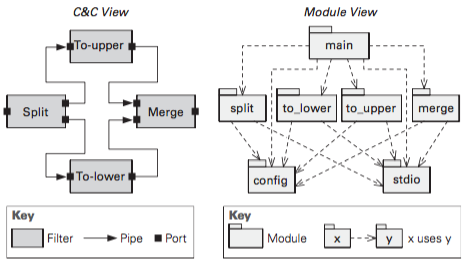
\includegraphics[width=100mm]{pipes-and-filters}
	\end{center}
	
		
    \optionA{The Merge component executes the module merge.}
    \optionB{The Merge component executes the modules merge and stdio.}
    \optionC{The module main is executed in the Merge component.}
    \optionD{The Pipe connectors do not execute any module.}
 \putOptions 
\end{ClosedQuestion}
}


% Component-and-Connector Styles

\newcommand{\qCCStyleOne}{
\begin{ClosedQuestion}
	When describing their system people refer to a part of it as containing a database server. Applying the component-and-connector styles learned in the course we can say that this system uses

    \optionA{A client-server style.}
    \optionB{A shared-data style.}
    \optionC{Both, client-server and shared-data styles.}
    \optionD{A blackboard style.}
 \putOptions 
\end{ClosedQuestion}
}

\newcommand{\qCCStyleTwo}{
\begin{ClosedQuestion}
	Consider the peer-to-peer architectural style
		
    \optionA{All the peers are equal.}
    \optionB{Any peer can access any other peer.}
    \optionC{Peers are only used to share files.}
    \optionD{The interaction between peers is symmetric.}
 \putOptions 
\end{ClosedQuestion}
}

\newcommand{\qCCStyleThree}{
\begin{ClosedQuestion}
	Consider the shared-data style. Which of the following qualities does it support?

    \optionA{Modifiability, because the Data Accessors do not depend on the data model.}
    \optionB{Scalability of read requests, because it is easy add more repositories to where reads are distributed, though there may be some level of inconsistency.}
    \optionC{Scalability of write requests, because a transactional system will synchronize the writes among the several repositories.}
    \optionD{Confidentially of data, because it can be replicated in several repositories.}
 \putOptions 
\end{ClosedQuestion}
}





% Component-and-Connector styles

%1
\newcommand{\qComponentAndConnectorOneOne}{
\begin{ClosedQuestion}
	Consider the Service-Oriented Architecture architectural style
		
    \optionA{The main quality this style addresses is interoperability.}
    \optionB{It cannot be applied when the system includes legacy systems.}
    \optionC{Its enterprise service bus cannot support asynchronous communication between the components.}
    \optionD{The typical communication pattern is point-to-point.}
 \putOptions 
\end{ClosedQuestion}
}

%2
\newcommand{\qComponentAndConnectorTwoOne}{
\begin{ClosedQuestion}
	Consider the following view of the Adventure Builder system
	
	\begin{center}
		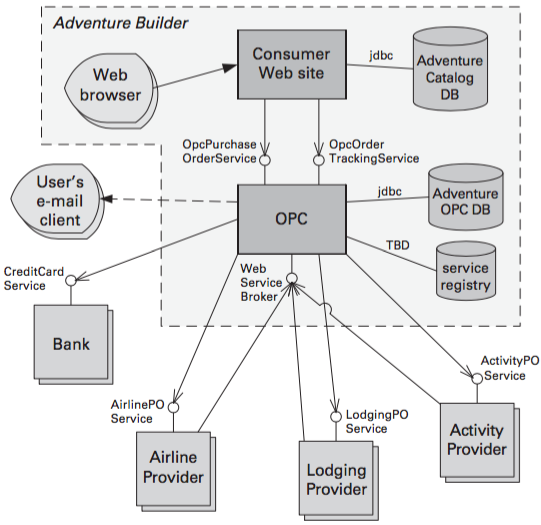
\includegraphics[width=80mm]{AdventureBuilder-SOA}
	\end{center}
	
	In this view the following architectural styles are used
	
		
    \optionA{Service-oriented architecture, and Client-server.}
    \optionB{Service-oriented architecture, and Shared-data.}
    \optionC{Service-oriented architecture, Shared-data, and Peer-to-peer.}
    \optionD{Service-oriented architecture, Shared-data, Peer-to-peer, and Client-server.}
 \putOptions 
\end{ClosedQuestion}
}
	
%3
\newcommand{\qComponentAndConnectorThreeOne}{
\begin{ClosedQuestion}
	Consider the following view of the Adventure Builder system
	
	\begin{center}
		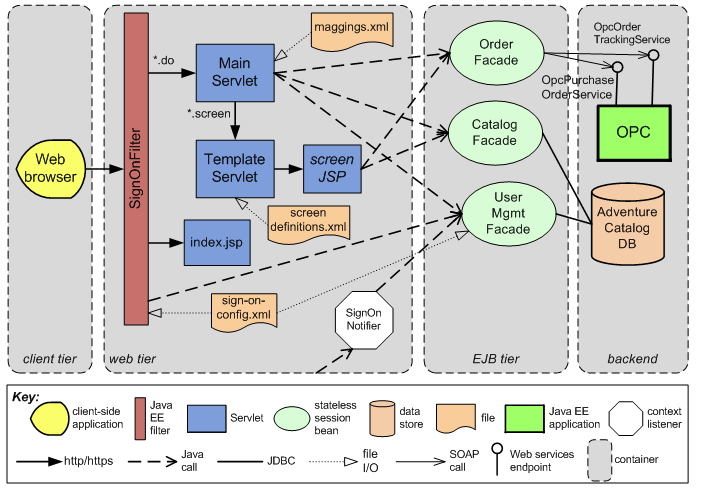
\includegraphics[width=100mm]{AdventureBuilder-Tiers}
	\end{center}
	
	In this view the following architectural styles are used
		
    \optionA{Tiers.}
    \optionB{Tiers, and Shared-data.}
    \optionC{Tiers, Shared-data, and Service-oriented architecture.}
    \optionD{Tiers, Shared-data, Service-oriented architecture, and Client-server.}
 \putOptions 
\end{ClosedQuestion}
}

% Allocation viewtype

%4
\newcommand{\qAllocationOne}{
\begin{ClosedQuestion}
	Consider the work assignment architectural style of the allocation viewtype.
			
    \optionA{It assigns components and connectors to people and teams.}
    \optionB{It is useful for the project managers.}
    \optionC{It does not consider the software that is outsourced.}
    \optionD{It allows to estimate the cost of hardware.}
 \putOptions 
\end{ClosedQuestion}
}

%5
\newcommand{\qAllocationTwo}{
\begin{ClosedQuestion}
	Consider the deployment architectural style of the allocation viewtype.
			
    \optionA{It assigns modules to the hardware.}
    \optionB{It cannot assign software elements to virtual servers because they are not hardware.}
    \optionC{For each set of software elements there is a single possible assignment to hardwre.}
    \optionD{It is useful for system administrators.}
 \putOptions 
\end{ClosedQuestion}
}

%6
\newcommand{\qAllocationThree}{
\begin{ClosedQuestion}
	Consider the install architectural style of the allocation viewtype.
			
    \optionA{The development team is the main stakeholder interesting in these views.}
    \optionB{It assigns modules to files.}
    \optionC{It is completely independent of the deployment architectural style.}
    \optionD{It helps on the configuration of systems.}
 \putOptions 
\end{ClosedQuestion}
}

% Infinispan views

%7
\newcommand{\qInfinispanOne}{
\begin{ClosedQuestion}
	Consider the Infinispan system when it is configured as a remote data grid. The relation between the Applications and the Grid is
			
    \optionA{Client-server.}
    \optionB{Peer-to-peer.}
    \optionC{Master-slave.}
    \optionD{Pipe-and-filter.}
 \putOptions 
\end{ClosedQuestion}
}

%8
\newcommand{\qInfinispanTwo}{
\begin{ClosedQuestion}
	In the description of Infinispan system can be read
	
	\begin{quote}
		Infinispan supports several pluggable cache stores-adapters that can be used to persist data to disk or any form of secondary storage. The current default implementation is a simplistic hash bucket and linked list implementation, where each hash bucket is represented by a file on the filesystem. While easy to use and configure, this isn't the best-performing implementation.
	\end{quote}
	
	The architectural style(s) that should be used to illustrate the sentence is (are)
			
    \optionA{Decomposition.}
    \optionB{Generalization.}
    \optionC{Decomposition and Generalization.}
    \optionD{Peer-to-peer.}
 \putOptions 
\end{ClosedQuestion}
}

%9
\newcommand{\qInfinispanThree}{
\begin{ClosedQuestion}
	In the description of Infinispan system can be read
	
	\begin{quote}
		When dealing with thread pools to process such asynchronous tasks, there is always a context switching overhead. That threads are not cheap resources is also noteworthy. Allocating appropriately sized and configured thread pools is important to any installation making use of any of the asynchronous features of Infinispan.
	\end{quote}
	
	The architectural style that should be used to illustrate the sentence is
			
    \optionA{Client-server.}
    \optionB{Communicating processes.}
    \optionC{Peer-to-peer.}
    \optionD{Shared-data.}
 \putOptions 
\end{ClosedQuestion}
}

% Micro-services and Amazon Cloud

%10
\newcommand{\qMicroAndAmazonOne}{
\begin{ClosedQuestion}
	Consider the following distinction between Monoliths and Microservices made by Matin Fowler
	
	\begin{center}
		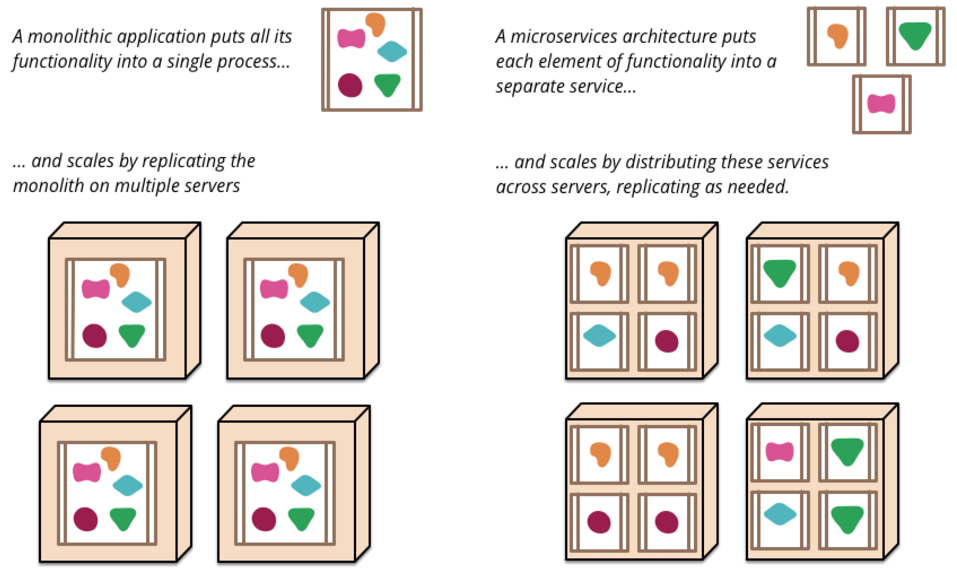
\includegraphics[width=100mm]{MonolithsVsMicroservices}
	\end{center}
	
	If we try to map this figure into a set of views we will need.
			
    \optionA{A decomposition view.}
    \optionB{A view of the component-and-connector viewtype.}
    \optionC{A view of the component-and-connector viewtype and a deployment view.}
    \optionD{A decomposition view, a view of the component-and-connector viewtype and a deployment view.}
 \putOptions 
\end{ClosedQuestion}
}

%11
\newcommand{\qMicroAndAmazonTwo}{
\begin{ClosedQuestion}
	Consider the following representation of Amazon's architecture (sorry for the figure's layout: \textbf{save trees})
			
	\begin{center}
		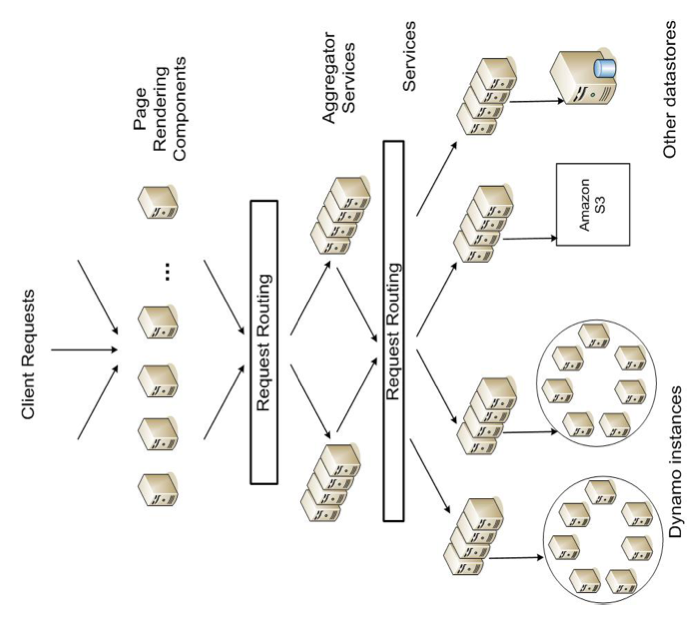
\includegraphics[width=80mm]{AmazonArchitecture}
	\end{center}
	
	What is the most relevant architecture style that is used in this figure?
	
    \optionA{Client-server to represent performance.}
    \optionB{Tiers to represent scalability.}
    \optionC{Service-oriented architecture to represent interoperability.}
    \optionD{Shared-data to represent modifiability.}
 \putOptions 
\end{ClosedQuestion}
}

%12
\newcommand{\qMicroAndAmazonThree}{
\begin{ClosedQuestion}
	In the interview Werner Vogels from Amazon gives to Jim Gray, Werner Vogels says that
	
	\begin{quote}
		The stored data formats are decoupled from the format in which you communicate data items. If there is no need for sharing schemas of the actual storage layout, you can focus on making sure that the service interfaces can evolve in a way that allows you to handle variations of data formats. 
	\end{quote}
	
	Which means that in the software architecture of Amazon's systems
			
    \optionA{The data-shared architectural style is not applied because data is encapsulated inside services.}
    \optionB{The sharing of data is done using a service-oriented architecture.}
    \optionC{Modifiability is not a concern of their architecture.}
    \optionD{The decouple of data formats does not support scalability because of the transactional properties.}
 \putOptions 
\end{ClosedQuestion}
}

% Jenkings views

%13
\newcommand{\qJenkinsOne}{
\begin{ClosedQuestion}
	Consider the following representation of the Buildbot system.
	
	\begin{center}
		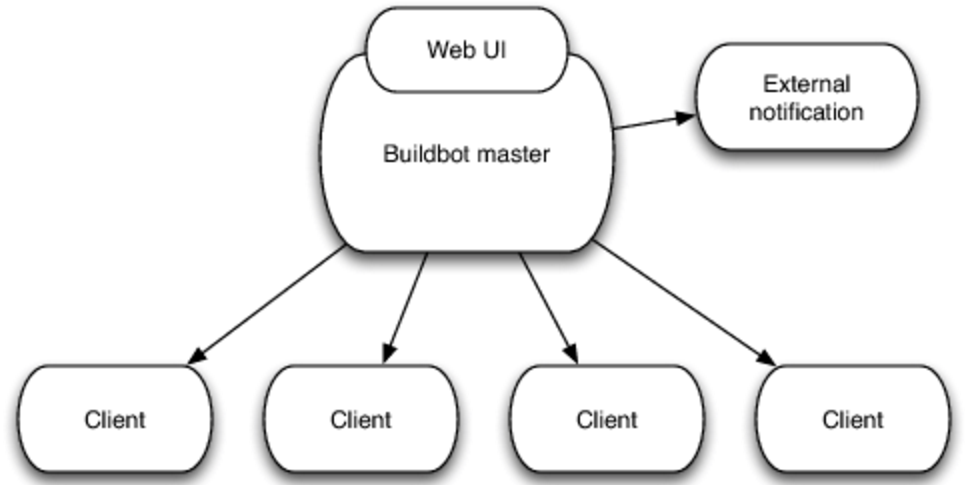
\includegraphics[width=80mm]{BuildbotArchitecture}
	\end{center}
	
	The architecture style between the Buildbot Master and the Clients is:
			
    \optionA{Peer-to-peer.}
    \optionB{Shared-data where the Buildbot is the data accessor.}
    \optionC{Client-server where the Buildbot is the client.}
    \optionD{Client-server where the Buildbot is the server.}
 \putOptions 
\end{ClosedQuestion}
}

%14
\newcommand{\qJenkinsTwo}{
\begin{ClosedQuestion}
	In the Continuous Integration case can be read
	\begin{quote}
		Build notification: The outcomes of builds generally need to be communicated to interested clients, either via pull (Web, RSS, RPC, etc.) or push notification (e-mail, Twitter, etc.) This can include notification of all builds, or only failed builds, or builds that haven't been executed within a certain period.
	\end{quote}
		The architectural style used in push notifications is
			
    \optionA{Publish-subscribe.}
    \optionB{Client-server.}
    \optionC{Shared-date.}
    \optionD{Generalization.}
 \putOptions 
\end{ClosedQuestion}
}

%15
\newcommand{\qJenkinsThree}{
\begin{ClosedQuestion}
	Consider the following representation of the CDash system
	
	\begin{center}
		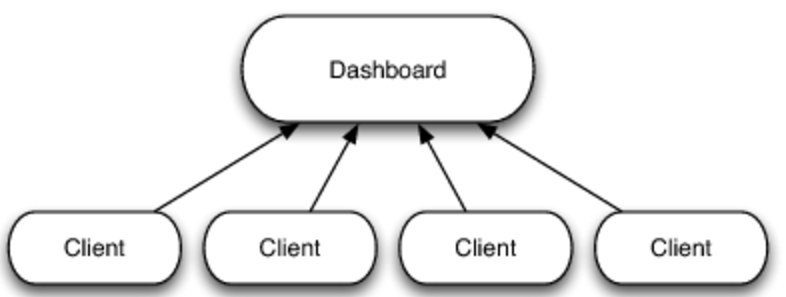
\includegraphics[width=80mm]{DashArchitecture}
	\end{center}
	
	The architecture style between the Dashboard and the Clients is:
			
    \optionA{Peer-to-peer.}
    \optionB{Shared-data where the Dashboard is the repository.}
    \optionC{Client-server where the Dashboard is the client.}
    \optionD{Client-server where the Dashboard is the server.}
 \putOptions 
\end{ClosedQuestion}
}



% Tiers, Dynamic reconfiguration, Peer-to-peer, Publish-subscribe

%1
\newcommand{\qPeerToPeerSpace}{
\begin{ClosedQuestion}
	The Peer-to-Peer architectural style provides high scalability and availability. In the context of a file sharing system  
	

    \optionA{The file transfers follows the same path of nodes used to identify where the file was located.}
    \optionB{The peer initiating the request for a file needs to know where the file is located.}
    \optionC{If a peer providing a file crashes it is necessary to restart to download the file from the begin.}
    \optionD{The price for high scalability and availability is the need to have several replicas of the files to be shared.}
 \putOptions
\end{ClosedQuestion}
}

%2
\newcommand{\qPeerToPeerDynamicReconfiguration}{
\begin{ClosedQuestion}
	In the description of the Gnutella system can be read:
	
	\begin{quote}
		The topology of the system changes at runtime as peer components connect and disconnect to the network.
	\end{quote}
	

    \optionA{When a peer connects to the network it establishes connections with all other peers in the network.}
    \optionB{The behavior described in the sentence can be represented in a view where the dynamic reconfiguration architectural style is used.}
    \optionC{When a peer receives a connection it sends all its files to the peer connecting it.}
    \optionD{The behavior described in the sentence can be represented in a view where the tier architectural style is used.}
 \putOptions
\end{ClosedQuestion}
}

%3
\newcommand{\qTiers}{
\begin{ClosedQuestion}
	The Tiers architectural style
	

    \optionA{It applies layers to tiers.}
    \optionB{Restrict the communication between components because, for instance, a group of components should be located in the same hardware.}
    \optionC{Is an extension of the Client-Server architectural style.}
    \optionD{Defines tiers as components.}
 \putOptions
\end{ClosedQuestion}
}

%4
\newcommand{\qPublishSubscribe}{
\begin{ClosedQuestion}
	In the Publish-Subscribe architectural style 
	

    \optionA{A component can subscribe to events.}
    \optionB{All the published events are received by their subscribing components.}
    \optionC{The events should be delivered by the same order they are sent.}
    \optionD{The set of events types are predefined at initialization time.}
 \putOptions
\end{ClosedQuestion}
}


% SOA, Pipes-and-Filters

%5 
\newcommand{\qSOAInteroperability}{
\begin{ClosedQuestion}
	The Service-Oriented Architecture style improves interoperability because
	

    \optionA{It enforces the use of a single implementation language among all applications.}
    \optionB{The orchestration is in charge of improving the transparent location of service providers.}
    \optionC{The enterprise service bus coordinates the execution of several services.}
    \optionD{It decouples applications developed for different organizations.}
 \putOptions
\end{ClosedQuestion}
}

%6 
\newcommand{\qSOAQualities}{
\begin{ClosedQuestion}
	The Service-Oriented Architecture style improves modifiability because
	

    \optionA{It encapsulates applications through well-defined interfaces.}
    \optionB{It decouples the coordination of the interaction among applications from the applications themselves.}
    \optionC{It improves transparency of location of service providers.}
    \optionD{It encapsulates applications through well-defined interfaces, decouples the coordination of the interaction among applications from the applications themselves, and improves transparency of location of service providers.}
 \putOptions
\end{ClosedQuestion}
}

%7
\newcommand{\qSOAClientServerPeertoPeer}{
\begin{ClosedQuestion}
	The Service-Oriented Architecture style
	

    \optionA{Is a Client-Server style because consumers are clients and providers are servers.}
    \optionB{Is a Peer-to-Peer style because consumers and providers are peers.}
    \optionC{Can use a Service Registry to improve transparency of location of service providers.}
    \optionD{Is a Publish-subscriber style because consumers use an enterprise service bus.}
 \putOptions
\end{ClosedQuestion}
}

%8
\newcommand{\qPipeFilterComposition}{
\begin{ClosedQuestion}
	The Pipe-and-Filter style allows composition of filters 
	

    \optionA{But when the filters are executed sequentially the composition power is reduced.}
    \optionB{Which improves modifiability, because filters are decoupled through pipes.}
    \optionC{But the size of buffers may reduce the composition power.}
    \optionD{And filters do not have to agree on the data formats.}
 \putOptions
\end{ClosedQuestion}
}

% Graphite views

%9
\newcommand{\qGraphiteDecompositionMemcached}{
\begin{ClosedQuestion}
	Consider the following decomposition view of the Graphite system where module \textsc{Store Graphs} is responsible for managing the storage of datapoints and graphs and module \textsc{Present Graphs} for graphs generation and presentation. Memcache is a library that maintains datapoints in memory to reduce the overhead of obtaining them from the file system.
	
	\centering
	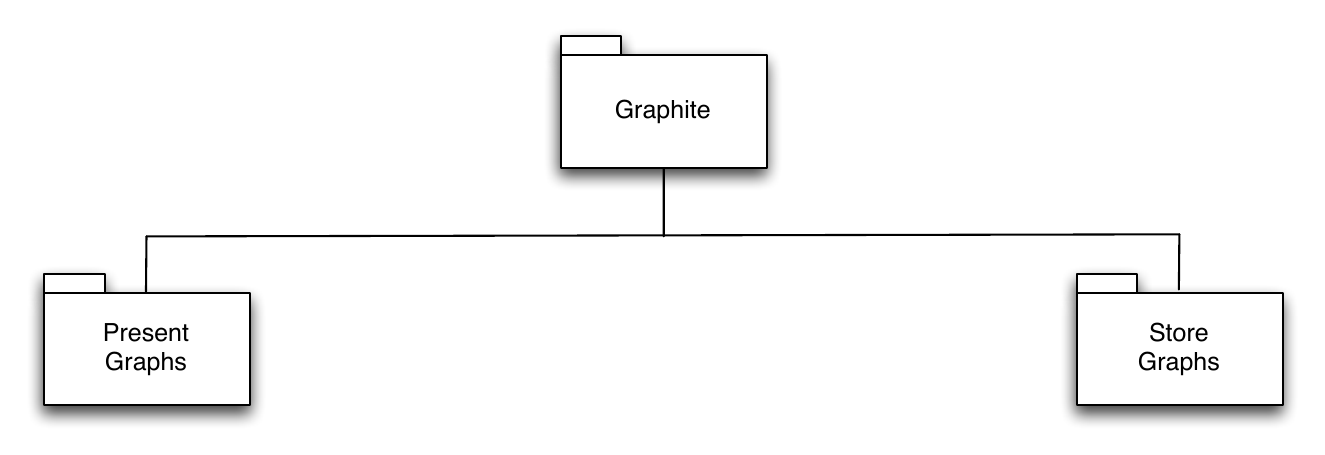
\includegraphics[width=100mm]{x-top-decomposition}

    \optionA{Memcached can be considered a sub-module of the Store Graphs module.}
    \optionB{Memcached can be considered a sub-module of the Present Graphs module.}
    \optionC{Memcached can be considered a direct sub-module of the top Graphite module.}
    \optionD{Memcached is not a module.}
 \putOptions
\end{ClosedQuestion}
}

%10
\newcommand{\qGraphiteDecompositionBuffering}{
\begin{ClosedQuestion}
	Consider the following decomposition view of the Graphite system where module \textsc{Store Graphs} is responsible for managing the storage of datapoints and graphs and module \textsc{Present Graphs} for graphs generation and presentation. Buffering is a library used to temporarily store incoming data point.
	
	\centering
	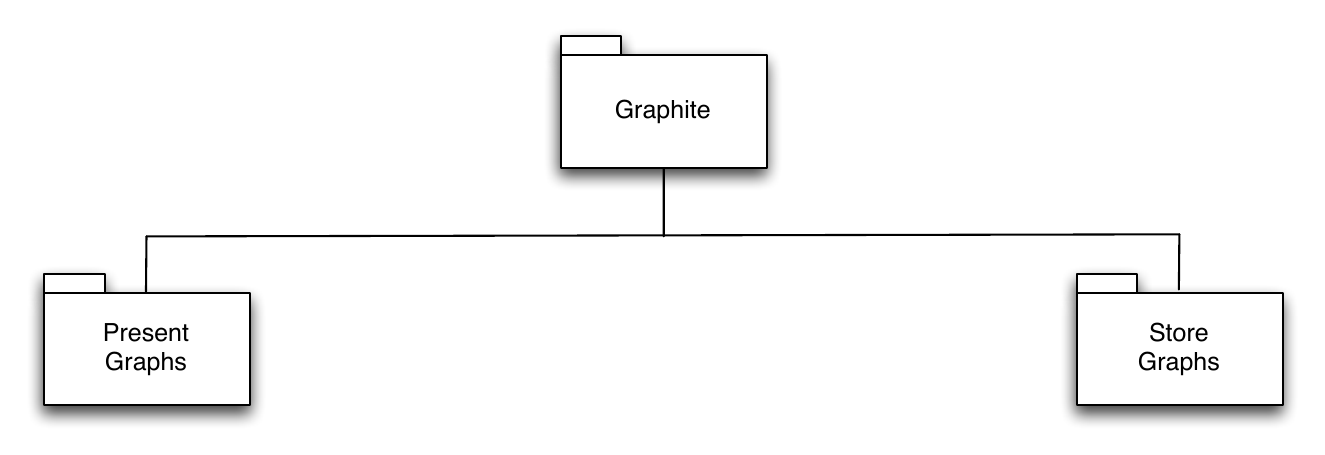
\includegraphics[width=100mm]{x-top-decomposition}

    \optionA{Buffering can be considered a sub-module of the Store Graphs module.}
    \optionB{Buffering can be considered a sub-module of the Present Graphs module.}
    \optionC{Buffering can be considered a direct sub-module of the top Graphite module.}
    \optionD{Buffering is not a module.}
 \putOptions
\end{ClosedQuestion}
}

%11
\newcommand{\qGraphiteCarbon}{
\begin{ClosedQuestion}
	Consider the following application-specific types that were defined for a component-and-connector view that depicts the components within \texttt{Carbon} component. 
	
	\centering
	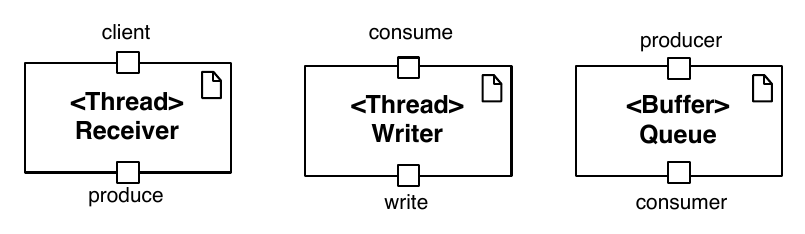
\includegraphics[width=100mm]{x-carbon-buffering}

    \optionA{In the view there are multiple instances of the \texttt{Queue} component.}
    \optionB{In the view there are multiple instances of the \texttt{Writer} component.}
    \optionC{In the view \texttt{Receiver} component's \texttt{client} port is not associated with an external port.}
    \optionD{In the view the \texttt{produce} port of a \texttt{Receiver} component is attached to the \texttt{consume} port of a \texttt{Writer} component.}
 \putOptions
\end{ClosedQuestion}
}


%12
\newcommand{\qGraphiteDataPointSocket}{
\begin{ClosedQuestion}
	Consider the following application-specific types. Note that \texttt{Queue} components are within the \texttt{Carbon} components. In a view that contains components of these three types 
	
	\centering
	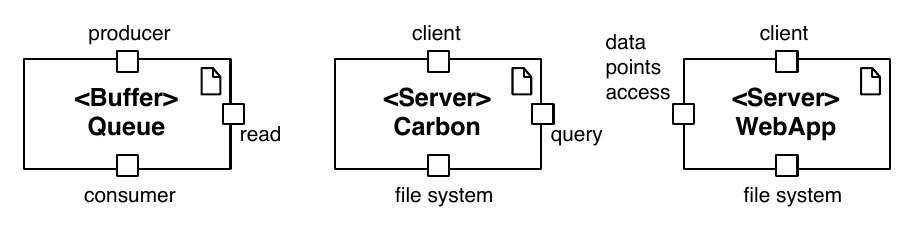
\includegraphics[width=120mm]{x-datapoint-access}

    \optionA{There is a message passing connector between the \texttt{read} port of \texttt{Queue} and the \texttt{data points access} port of \texttt{WebApp}.}
    \optionB{There is a interface delegation relation between the \texttt{read} port of \texttt{Queue} and the \texttt{query} port of \texttt{Carbon}.}
    \optionC{There is a connector between the \texttt{producer} port of a \texttt{Queue} component and the \texttt{client} port of its \texttt{Carbon} component.}
    \optionD{The \texttt{client} ports of \texttt{Carbon} and \texttt{WebApp} are connected to a \texttt{Client} component through the same connector instance.}
 \putOptions
\end{ClosedQuestion}
}


% Allocation viewtype

%13
\newcommand{\qAllocationStylesCost}{
\begin{ClosedQuestion}
	Consider a stakeholder that is particularly concerned about the total cost of the project. When it comes to describing the system using allocation viewtypes is interested in

    \optionA{A deployment view.}
    \optionB{A work assignment view.}
    \optionC{A deployment and a work assignment view.}
    \optionD{A install view.}
 \putOptions
\end{ClosedQuestion}
}

%14
\newcommand{\qImplementationStyle}{
\begin{ClosedQuestion}
	An architecture can also be represented by the set of files which contains its modules code. A suitable architectural style to represent this set of files is

    \optionA{Deployment style.}
    \optionB{Implementation style.}
    \optionC{Install style.}
    \optionD{Work assignment style.}
 \putOptions
\end{ClosedQuestion}
}

%15
\newcommand{\qInstallStyle}{
\begin{ClosedQuestion}
	An important stage of the development of any system is its build into the set of executable files. A suitable architectural style which helps on the definition of the build process is

    \optionA{Deployment style.}
    \optionB{Implementation style.}
    \optionC{Install style.}
    \optionD{Work assignment style.}
 \putOptions
\end{ClosedQuestion}
}

%16
\newcommand{\qDeploymentStyleLimitExposure}{
\begin{ClosedQuestion}
	An architect needs to show that a security tactic of limit exposure will be effectively provided by the executing system. Therefore, she decides to design
	
    \optionA{A work assignment view.}
    \optionB{A deployment view.}
    \optionC{An install view.}
    \optionD{An implementation view.}
 \putOptions
\end{ClosedQuestion}
}


% DVD Catalog

%17
\newcommand{\qDVDCatalogMeta}{
\begin{ClosedQuestion}
	Consider the module viewtype views of the DVDCatalog application. The architect knows about a new requirement 
	
	\begin{quote}
		The application should support other kinds of catalogs (CDs, games, books, ...). 
	\end{quote}
	
	This requirement requires a change of
	
    \optionA{The layered view to support a new specific layer for the customization of the catalog.}
    \optionB{The layered view to accommodate a new layer for which kind of catalog, which other layers may use.}
    \optionC{The data model view in order to define entities for each kind of catalog.}
    \optionD{The data model view in order to define generic entities that can be customized for different kinds of catalogs.}
 \putOptions
\end{ClosedQuestion}
}

%18
\newcommand{\qDVDCatalogAspects}{
\begin{ClosedQuestion}
	Consider the module viewtype views of the DVDCatalog application. The architect knows about a new requirement 
	
	\begin{quote}
		To allow the share of catalogs with family and friends, including some access control. 
	\end{quote}
	
	This requirement requires 
	
    \optionA{A change to the uses view to represent that friends can use each other catalog.}
    \optionB{A change of the layered view to support different presentations, one for each friend.}
    \optionC{A change of the decomposition view to include the responsibilities associated with the access control.}
    \optionD{A new aspect view to include the responsibilities associated with the access control.}
 \putOptions
\end{ClosedQuestion}
}

%19
\newcommand{\qDVDCatalogMobile}{
\begin{ClosedQuestion}
	Consider the module viewtype views of the DVDCatalog application. The architect knows about a new requirement 
	
	\begin{quote}
		To support iPhone/iPad/Android version with sync, which allows offline use of the application in the mobile device and data synchronization to occur when a connection is available
	\end{quote}
	
	This requirement requires a change of
	
    \optionA{The decomposition view to include a module for the synchronization responsibilities.}
    \optionB{The uses view to represent how the mobile device uses the Catalog application.}
    \optionC{The layered view to include a layer for each type of device.}
    \optionD{The domain layer of the layered view to represent the types of devices.}
 \putOptions
\end{ClosedQuestion}
}

%20
\newcommand{\qDVDCatalogMultiPlatform}{
\begin{ClosedQuestion}
	Consider the module viewtype views of the DVDCatalog application. The architect knows about a new requirement 
	
	\begin{quote}
		To support multi-platform (Mac, Windows, Linux)
	\end{quote}
	
	This requirement requires a change of
	
    \optionA{The layered view to deal with the aspects of portability.}
    \optionB{The uses view to show the coupling between the different platforms.}
    \optionC{The uses view to show the uses relationships between the different platforms.}
    \optionD{The data model view to represent each one of the platforms.}
 \putOptions
\end{ClosedQuestion}
}



% Amazon Silk vs Google Chrome

%1
\newcommand{\qSilkMobileDevices}{
\begin{ClosedQuestion}
	When comparing Amazon Silk with Google Chrome in the context of mobile devices

    \optionA{Amazon Silk is more convenient for mobile devices because it does most of the computation in the cloud.}
    \optionB{Google Chrome is more convenient for mobile devices because it has an optimized network stack that runs in any kind device.}
    \optionC{Amazon Silk is more convenient for mobile devices because it customizes the number of threads that run in the device.}
    \optionD{Google Chrome is more convenient for mobile devices because content delivery is optimized.}
 \putOptions
\end{ClosedQuestion}
}

%2
\newcommand{\qSilkPredictor}{
\begin{ClosedQuestion}
	When comparing Amazon Silk with Google Chrome in the context of the prediction of pages the user is going to access
	
    \optionA{Amazon Silk predicts accesses based on the information gathered for all Silk users.}
    \optionB{Google Chrome uses a usability maintain system model tactic.}
    \optionC{Amazon Silk predictions are constrained by the amount of information it can store about each user access.}
    \optionD{Google Chrome predictions do not require storage in the client-side.}
 \putOptions
\end{ClosedQuestion}
}

%3
\newcommand{\qSilkCaching}{
\begin{ClosedQuestion}
	When comparing Amazon Silk with Google Chrome  

    \optionA{Amazon Silk explicitly caches pages on the browser to optimize accesses.}
    \optionB{Google Chrome predictor takes into consideration the amount of available cache.}
    \optionC{Amazon Silk cache is not shared between different users of the service to support confidentiality.}
    \optionD{Google Chrome cache is shared among the different users of a desktop machine.}
 \putOptions
\end{ClosedQuestion}
}

%4
\newcommand{\qSilkConnections}{
\begin{ClosedQuestion}
	When comparing Amazon Silk with Google Chrome  
	
    \optionA{In Amazon Silk a request for a web page corresponds to a peer-to-peer interaction between all the web components containing the resources.}
    \optionB{In Google Chrome a request for a web page is accomplished by a single access to the internet.}
    \optionC{In Amazon Silk a request for a web page corresponds to requesting a service from the amazon cloud.}
    \optionD{In Google Chrome a request for a web page aggregates the page on the background before it is sent to the client.}
 \putOptions
\end{ClosedQuestion}
}


% ThousandParsec views

%5 
\newcommand{\qThousandParsecAI}{
\begin{ClosedQuestion}
	Consider the architectural views for the ThousandParsec system. The following diagram depicts a fragment of a proposal for the decomposition view of the system. The AI players should be described
	
	\centering
	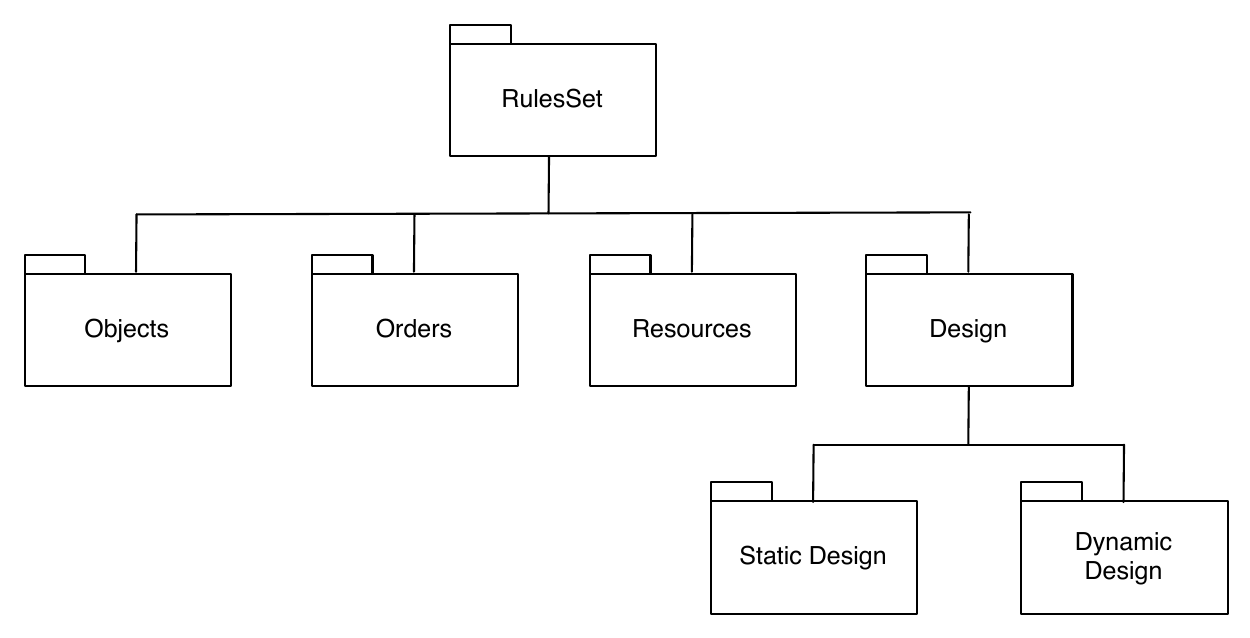
\includegraphics[width=100mm]{x-ThousandParsec-ruleset}

    \optionA{As a specialization of the RulesSet module.}
    \optionB{As a submodule of the RulesSet module.}
    \optionC{As a module but not included in the RulesSet subtree.}
    \optionD{As a specialization of the Design module.}
 \putOptions
\end{ClosedQuestion}
}

%6 
\newcommand{\qThousandParsecModule}{
\begin{ClosedQuestion}
	Consider the architectural views for the ThousandParsec system. The following diagram depicts a fragment of a proposal for the decomposition view of the system. The ThousandParsec protocol
	
	\centering
	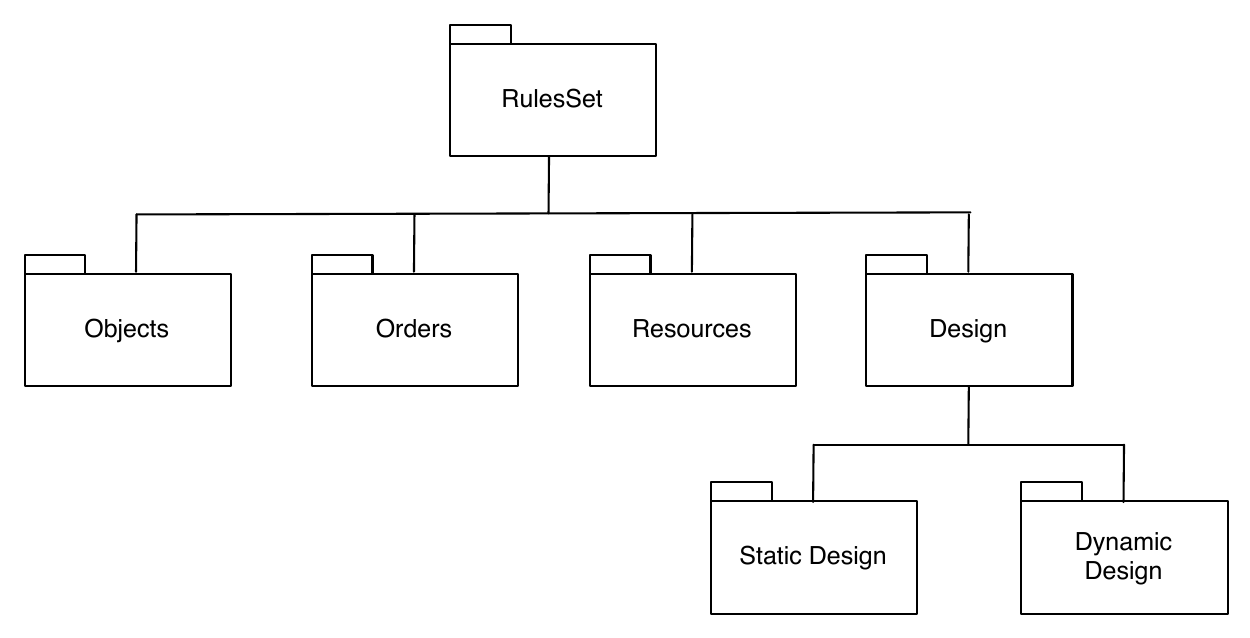
\includegraphics[width=100mm]{x-ThousandParsec-ruleset}

    \optionA{Should be described as a submodule of the RulesSet module.}
    \optionB{Should be described as a submodule of but not included in the RulesSet subtree.}
    \optionC{Should be described as a submodule of the Design module.}
    \optionD{Should not be described as a module because it is a component.}
 \putOptions
\end{ClosedQuestion}
}

%7 
\newcommand{\qThousandParsecTPConnector}{
\begin{ClosedQuestion}
	Consider the architectural views for the ThousandParsec system. The following diagram depicts a proposal of application-specific types for the architectural components, where the names of the ports are missing. Between the GameClient and GameServer components
	
	\centering
	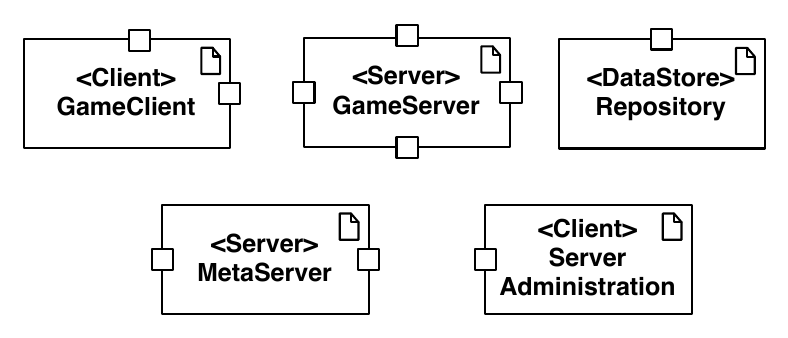
\includegraphics[width=80mm]{x-ThousandParsec-cc}

    \optionA{There is a ThousandParsec connector.}
    \optionB{There is a Request/Reply connector.}
    \optionC{There is a ThousandParsec connector which can be decomposed into a set of components and Request/Reply connectors.}
    \optionD{There is an EventBus connector.}
 \putOptions
\end{ClosedQuestion}
}

%8 
\newcommand{\qThousandParsecReadWriteConnector}{
\begin{ClosedQuestion}
	Consider the architectural views for the ThousandParsec system. The following diagram depicts a proposal of application-specific types for the architectural components, where the names of the ports are missing. Between the GameServer and Repository component
	
	\centering
	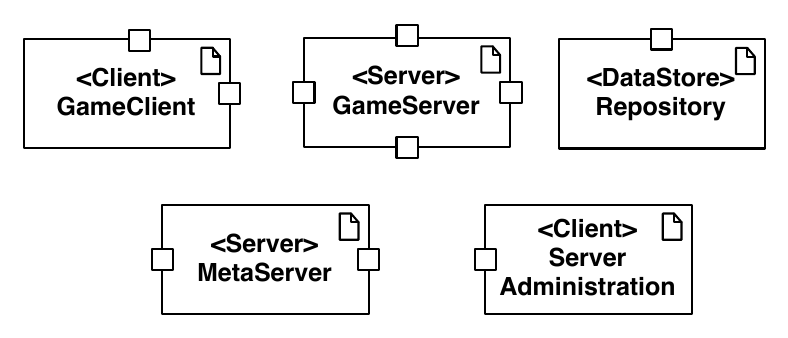
\includegraphics[width=80mm]{x-ThousandParsec-cc}

    \optionA{There is a ThousandParsec connector.}
    \optionB{There is a Read/Write connector which encapsulates a redundant Repository.}
    \optionC{There is a Read/Write connector which guarantees that players turns are not lost.}
    \optionD{There is a Read/Write connector which guarantees that only the turns of the last two players may be lost.}
 \putOptions
\end{ClosedQuestion}
}


% The architecture of OrderPad

%9
\newcommand{\qOrderPadPortability}{
\begin{ClosedQuestion}
	Consider the architecture of the Morrison's OrderPad. The decision between the use of a Native application or HTML5 on the implementation of the client in the Pad
	
    \optionA{Was taken because HTML5 provides better portability qualities.}
    \optionB{Was taken because Native applications provide better modifiability qualities.}
    \optionC{Was taken because HTML5 provides better usability qualities.}
    \optionD{Was taken because Native application provide better support for working offline.}
 \putOptions
\end{ClosedQuestion}
}

%10
\newcommand{\qOrderPadReliability}{
\begin{ClosedQuestion}
	Consider the architecture of the Morrison's OrderPad. The connector between the client component, executing in the Pad, and the server component, executing in the OrderPadDatabase
	
    \optionA{Supports asynchronous communication to deal with disconnected mode.}
    \optionB{Implements an event bus that allows the server to inform the client about new order recommendations.}
    \optionC{May loose some of the changes done on the client component.}
    \optionD{Has reduced reliability qualities.}
 \putOptions
\end{ClosedQuestion}
}

%11
\newcommand{\qOrderPadMainframeConnector}{
\begin{ClosedQuestion}
	Consider the architecture of the Morrison's OrderPad. The final interaction between the OrderPadDatabase component and Mainframe component is supported by 
	
    \optionA{Two distinct unidirectional connectors.}
    \optionB{A single bidirectional connector.}
    \optionC{Three distinct unidirectional connectors.}
    \optionD{A single unidirectional connector.}
 \putOptions
\end{ClosedQuestion}
}

%12
\newcommand{\qOrderPadIterative}{
\begin{ClosedQuestion}
	Consider the architecture of the Morrison's OrderPad. In the description of the system can be read:
	
	\begin{quote}
		One of these was using a file-transfer to send data to the mainframe rather than MQ, which wouldn't perform well once many stores were active.
	\end{quote}
	
	This approach means that
	
    \optionA{Performance was traded for easy of development.}
    \optionB{An iterative development was followed, which allowed more time to develop a connector with good performance in the latter stages of the project.}
    \optionC{Performance was traded for the modifiability quality.}
    \optionD{An incremental development was followed, which allowed to have the system in production without being necessary to export all the information to the mainframe.}
 \putOptions
\end{ClosedQuestion}
}


% SocialCalc Views

%13
\newcommand{\qSocialCalcRemoteCursor}{
\begin{ClosedQuestion}
	Consider the architectural views for the SocialCalc system. The following diagram depicts a proposal for a component-and-connector view of the client Spreadsheet. It can be read in the case description: \emph{A simple improvement is for each client to broadcast its cursor position to other users, so everyone can see which cells are being worked on.}
	
	\centering
	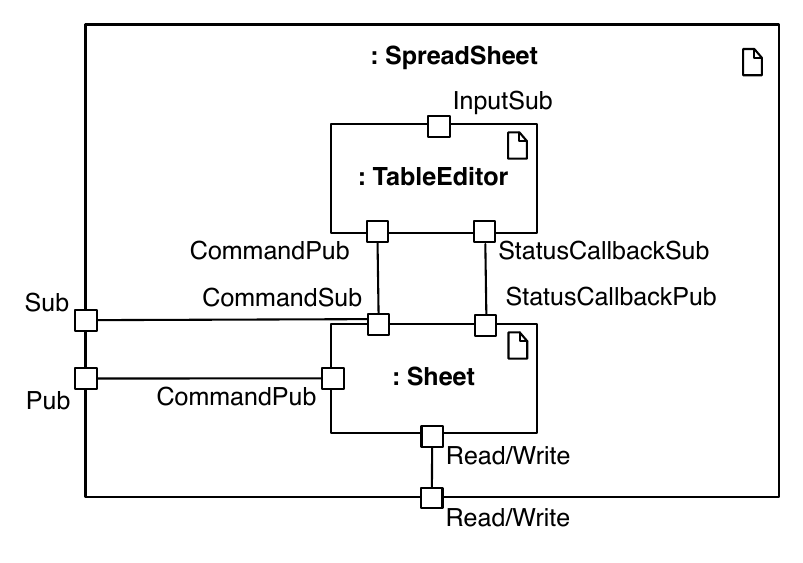
\includegraphics[width=80mm]{x-SocialCalc-cc-client}

    \optionA{The \textsc{: TableEditor} broadcasts the cursor position through the \textsc{: Sheet}.}
    \optionB{An interface delegation is missing in the picture to represent the \textsc{: TableEditor} broadcasting the cursor position through the \textsc{Pub} port.}
    \optionC{The \textsc{: Sheet} broadcasts the cursor position through the \textsc{Pub} port.}
    \optionD{The \textsc{: TableEditor} broadcasts the cursor position through its \textsc{: StatusCallback} port.}
 \putOptions
\end{ClosedQuestion}
}

%14
\newcommand{\qSocialCalcServer}{
\begin{ClosedQuestion}
	Consider the architectural views for the SocialCalc system. The following diagram depicts a proposal for a component-and-connector view of the system. According to this representation
	
	\centering
	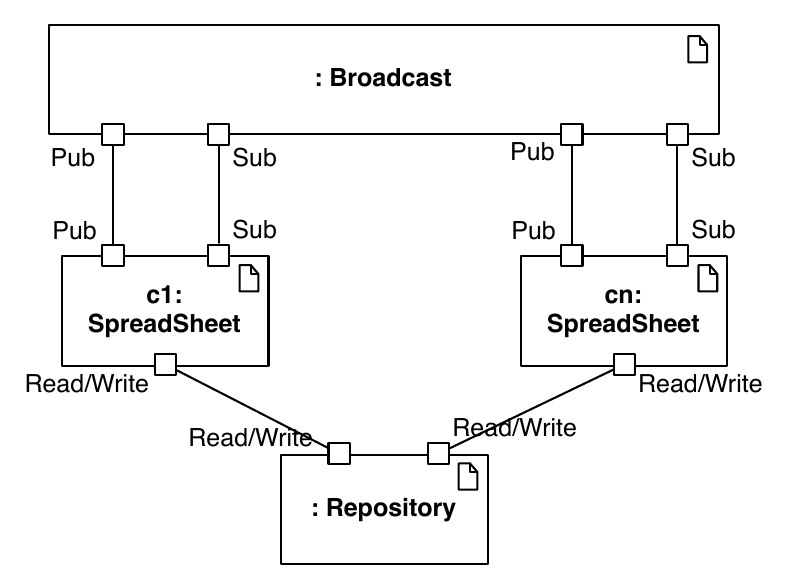
\includegraphics[width=80mm]{x-SocialCalc-cc}

    \optionA{The server implements the \textsc{: Repository} component and the \textsc{: Broadcast} connector.}
    \optionB{The server implements the \textsc{: Repository} component.}
    \optionC{The server implements the \textsc{: Broadcast} connector.}
    \optionD{The server implements the \textsc{SpreadSheet} components}
 \putOptions
\end{ClosedQuestion}
}

%15
\newcommand{\qSocialCalcParser}{
\begin{ClosedQuestion}
	Consider the architectural views for the SocialCalc system. The following diagram depicts a proposal for a component-and-connector view of the client Spreadsheet. A \textsc{Parser} module is used when loading a file
	
	\centering
	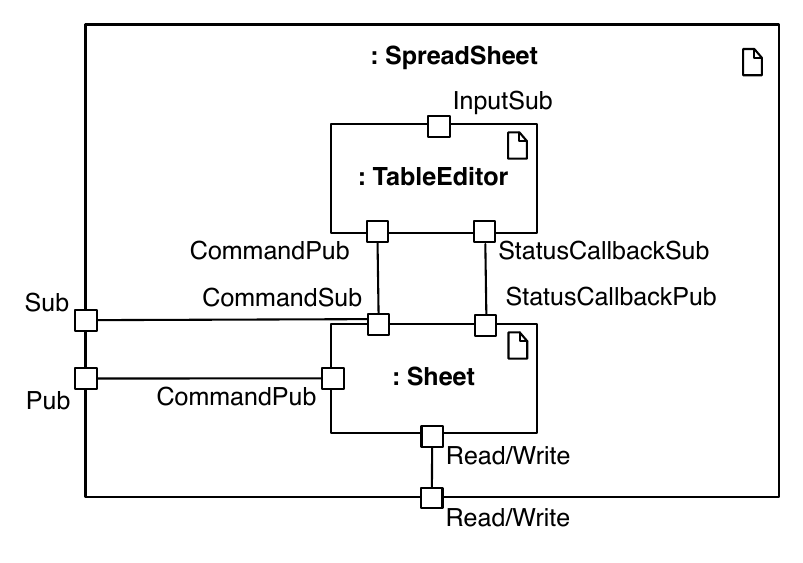
\includegraphics[width=80mm]{x-SocialCalc-cc-client}

    \optionA{The \textsc{Parser} module is part of the code executed by the \textsc{: TableEditor} component.}
    \optionB{The \textsc{Parser} module is part of the code executed by the \textsc{: Sheet} component.}
    \optionC{The code of the \textsc{Parser} module is executed by a repository component, which is not represented in the view.}
    \optionD{The code of the \textsc{Parser} module is executed by both, the \textsc{: Sheet} and the repository components (the latter is not visible in the view).}
 \putOptions
\end{ClosedQuestion}
}

%16
\newcommand{\qSocialCalcConflictResolution}{
\begin{ClosedQuestion}
	Consider the architectural views for the SocialCalc system. The following diagram depicts a proposal for a component-and-connector view of the client Spreadsheet. A \textsc{ConflictResolution} module is used when local commands conflict with remote commands.
	
	\centering
	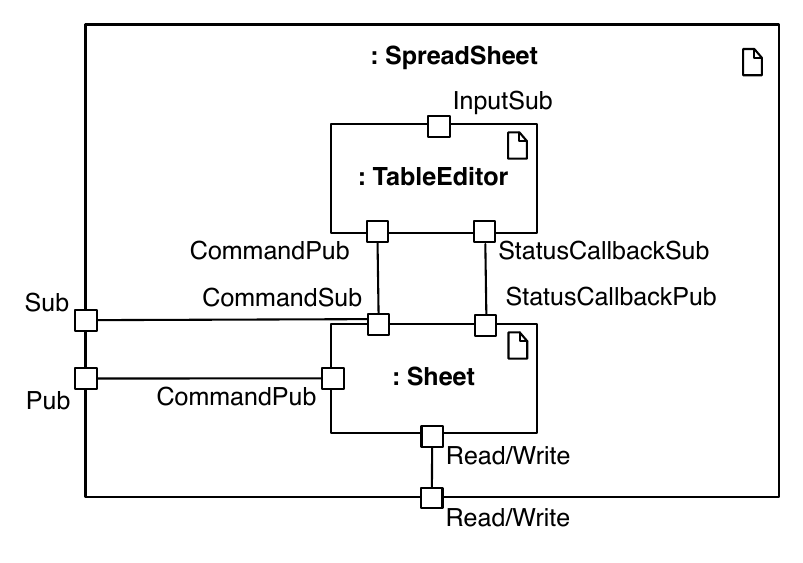
\includegraphics[width=80mm]{x-SocialCalc-cc-client}

    \optionA{The \textsc{ConflictResolution} module is part of the code executed by the \textsc{: TableEditor} component.}
    \optionB{The \textsc{ConflictResolution} module is part of the code executed by the \textsc{: Sheet} component.}
    \optionC{The code of the \textsc{ConflictResolution} module is executed by a broadcast connector that implements an eventbus between the \textsc{SpreadSheet} components.}
    \optionD{The code of the \textsc{ConflictResolution} module is executed in a server component because it needs to be centralized.}
 \putOptions
\end{ClosedQuestion}
}


% Domain Logic and Access Patterns

%17
\newcommand{\qLogicAccessDomainModel}{
\begin{ClosedQuestion}
	When the domain logic is organized using a Domain Model pattern the most suitable data source patterns are

    \optionA{Table Data Gateway and Row Data Gateway.}
    \optionB{Row Data Gateway and Active Record.}
    \optionC{Row Data Gateway and Data Mapper.}
    \optionD{Active Record and Data Mapper.}
 \putOptions
\end{ClosedQuestion}
}

%18
\newcommand{\qLogicAccessTransactionScript}{
\begin{ClosedQuestion}
	When the domain logic is organized using a Transaction Script pattern the most suitable data source patterns are

    \optionA{Table Data Gateway and Row Data Gateway.}
    \optionB{Row Data Gateway and Active Record.}
    \optionC{Row Data Gateway and Data Mapper.}
    \optionD{Active Record and Data Mapper.}
 \putOptions
\end{ClosedQuestion}
}

%19
\newcommand{\qLogicAccessTransactionScriptDomainObjects}{
\begin{ClosedQuestion}
	When the domain logic is organized using a Transaction Script pattern the domain objects

    \optionA{Are responsible for loading the objects they refer to.}
    \optionB{Are responsible for the management of transactions, begin and end of transactions.}
    \optionC{Contain the business logic.}
    \optionD{May not even exist, only record sets are used.}
 \putOptions
\end{ClosedQuestion}
}

%20
\newcommand{\qLogicAccessTableModule}{
\begin{ClosedQuestion}
	When the domain logic is organized using a Table Module pattern 

    \optionA{An object oriented style is followed.}
    \optionB{The business logic is organized around record sets.}
    \optionC{Row Data Gateway is the most suitable data source pattern.}
    \optionD{A Service Layer should be used to provide an interface for the presentation layer.}
 \putOptions
\end{ClosedQuestion}
}





%%% EXAMS

%1 Architecture Influence Cycle
\newcommand{\qArchitectureInfluenceCycleOne}{
\begin{ClosedQuestion}
	Consider the following sentence by Melvin Conways, also known as Conway's Law
	
	\begin{quote}
		organizations which design systems ... are constrained to produce designs which are copies of the communication structures of these organizations
	\end{quote}
		
    \optionA{This law highlights the impact of the business on the architecture}
    \optionB{This law can be seen as an example of the architecture influence cycle}
    \optionC{This law states that architectures impact on the structure of the organization}
    \optionD{This law does not apply to the design of architectures}
 \putOptions 
\end{ClosedQuestion}
}


\newcommand{\qArchitectureInfluenceCycleTwo}{
\begin{ClosedQuestion}
  	  Designing the software architecture for a complex system

   	 \optionA{Is useful only if done (even if only partially) before the
	 	system's implementation is concluded, given that the architecture
    	is used for restricting the implementation}
	\optionB{Is useful only if done (even if only partially) before the
    	system's implementation is concluded, because if the system is
    	already implemented, its implementation uniquely determines the
    	architecture}
    \optionC{Is useful only if done (even if only partially) before the
    	system passes all of the acceptance tests by the client, given
    	that no more requirements changes will take place after that time}
    \optionD{Is useful even if the implementation is concluded and the
    	system has entered the maintenance phase}
		
    \putOptions %D
\end{ClosedQuestion}
}


%2 Adventure Builder - NEW
\newcommand{\qAdventureBuilderOne}{
\begin{ClosedQuestion}
  	Consider the following architectural view of the Adventure Builder system
	
	\begin{center}
		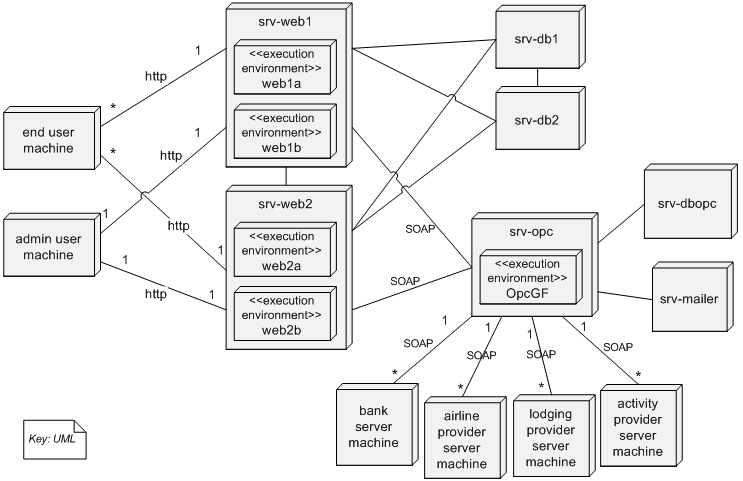
\includegraphics[width=80mm]{../AdventureBuilderDeployment}
	\end{center}
	
	According to this view the stakeholders can see that the Adventure Builder system

   	\optionA{Becomes unavailable for clients if there is a fault in the hardware of web server (srv-web)}
	\optionB{Becomes unavailable for clients if there is a fault in the hardware of database server (srv-db)}
    \optionC{Becomes unavailable for clients if there is a fault in the hardware of service server (srv-opc)}
    \optionD{Becomes unavailable for banks if there is a fault in the hardware of service server (srv-opc)}
		
    \putOptions
\end{ClosedQuestion}
}

%2 Adventure Builder - NEW
\newcommand{\qAdventureBuilderTwo}{
\begin{ClosedQuestion}
  	Consider the following architectural view of the Adventure Builder system
	
	\begin{center}
		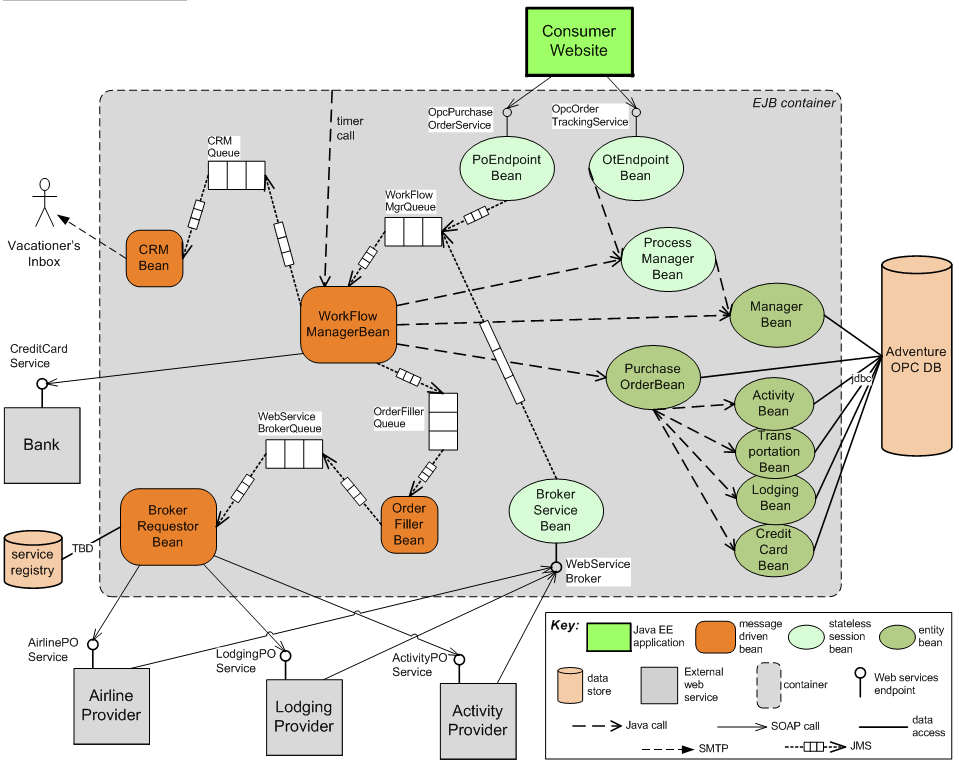
\includegraphics[width=120mm]{../AdventureBuilderComponentConector}
	\end{center}
	
	In this component-and-connector view the interactions the interactions between components follow the architectural style(s)

   	\optionA{Communicating processes}
	\optionB{Communicating processes and shared-data}
    \optionC{Communicating processes, shared-data and service-oriented architecture}
    \optionD{Communicating processes, shared-data, service-oriented architecture, and peer-to-peer}
		
    \putOptions %D
\end{ClosedQuestion}
}



%3 Featuritis Performitis Flexibilities
\newcommand{\qRequirementsOne}{
\begin{ClosedQuestion}
	Frank Buschmann cites the characterization Marquardt does of Performitis:
		
	\begin{quote}
		Each part of the system is directly influenced by local performance tuning measures. There is no global performance strategy, or it ignores other qualities of the system as testability and maintainability.
	\end{quote}
	
	From this problem you can conclude that:

    \optionA{Performance is a quality that you have to address at the end of the development process}
    \optionB{There is no system which can have good performance and be easily maintainable}
    \optionC{We have to distinguish architectural performance from opportunistic performance}
    \optionD{The system performance quality has impact on the performance of the execution of tests}
 \putOptions
\end{ClosedQuestion}
}

\newcommand{\qRequirementsTwo}{
\begin{ClosedQuestion}
  The architecturally significant requirements are important in the process of creating
  the software architecture for a system because they are

  \optionA{The most important requirements (both functional and
  	qualities) that the system must achieve}
  \optionB{The components that manage the communication between the
  	remaining elements in the system}
  \optionC{The stakeholders that drive the development of the system}
  \optionD{The tactics that satisfy the most important requirements for
  	the system}
  
 \putOptions
\end{ClosedQuestion}
}


%4 Architecture Definition
\newcommand{\qArchitectureDefinitionOne}{
	\begin{ClosedQuestion}
	    Consider that a software development team uses an agile methodology
	    such as XP (Extreme Programming), where no documentation is
	    produced.  Then, the systems developed by that team

	    \optionA{Typically have a software architecture that results
	      from the common knowledge about the system that is shared among
	      the team members}
	    \optionB{Do not have a software architecture, because in agile
	      methodologies there is no architectural design phase}
	    \optionC{Do not have a software architecture, because the practice of
	      refactoring allows changing every part of the system easily}
	    \optionD{May have a software architecture, but that architecture is
	      not known because it was neither designed nor documented}
	 	
    \putOptions
	\end{ClosedQuestion}
}

\newcommand{\qArchitectureDefinitionTwo}{
	\begin{ClosedQuestion}
	 	The software architecture of a system

    	\optionA{Depends mostly on the system's functional requirements}
    	\optionB{Depends more on the architect's experience than on anything else}
    	\optionC{Should not depend on the skills of the developing team}
    	\optionD{None of the above}
    \putOptions
	\end{ClosedQuestion}
}


%5 Module vs Component
\newcommand{\qModuleComponentOne}{
  \begin{ClosedQuestion}
    Consider the Figure that describes the use of
    caches in web services.  
	
	\begin{center}
		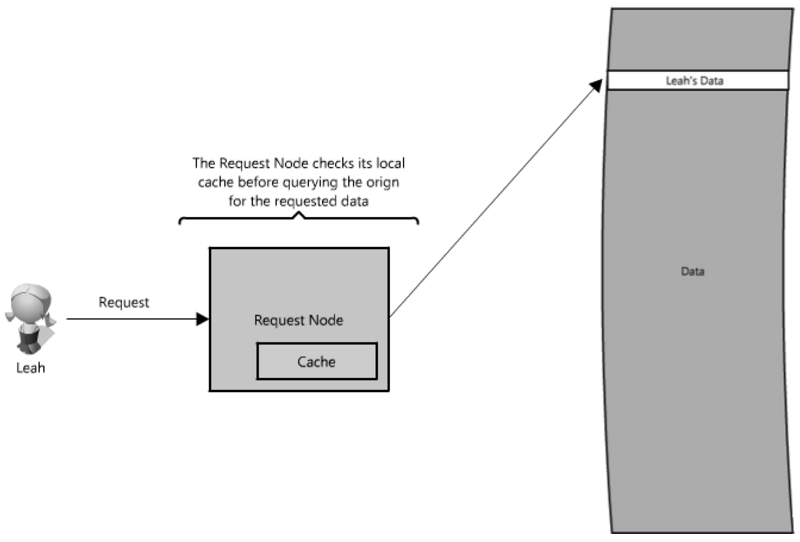
\includegraphics[width=80mm]{../RequestNodeCache}
	\end{center}
	
	In that Figure, there is a
    rectangle with the name \emph{Cache} within another rectangle with
    the name \emph{Request Node}.  Taking into account the description
    made in the text and the goal of that Figure, those rectangles
    correspond to which type of software elements?

    \optionA{They are both modules}
    \optionB{They are both components}
    \optionC{The \emph{Request Node} is a component and the
      \emph{Cache} is a module}
    \optionD{The \emph{Request Node} is a module and the \emph{Cache}
      is a component}
    \putOptions

% Resposta: B
  \end{ClosedQuestion}
}

\newcommand{\qModuleComponentTwo}{
 \begin{ClosedQuestion}
    Which of the following phrases best describe the relationship
    between modules and components?

    \optionA{A module may contain code from different components}
    \optionB{A component may execute code from different modules}
    \optionC{A module may execute code from different components}
    \optionD{A component may contain code from different modules}
    \putOptions

 \end{ClosedQuestion}
}


%6 Scenarios and Tactics
\newcommand{\qScenariosTacticsOne}{
\begin{ClosedQuestion}
  As part of the process of creating an architecture, we talked about
  a framework for capturing some of the requirements for a system.  In
  this context, \textbf{concrete scenarios} are used for

  \optionA{Describing what are the qualities that the system should possess}
  \optionB{Describing a set of steps that a user of the system must
  	perform to accomplish some task}
  \optionC{Describing a use case for the system that makes clear what
    should be the system's responses to each of the user's inputs}
  \optionD{Describing the system's features by way of different
    usage scenarios for it, in which users play the role of actors}
  \putOptions
\end{ClosedQuestion}
}

\newcommand{\qScenariosTacticsTwo}{
\begin{ClosedQuestion}
	General scenarios play an important role in the development of a software architecture
	because
	
	\optionA{They describe general requirements that all systems should try to satisfy}
	\optionB{They allow us to build a more robust architecture that satisfies less specific
		requirements, which address a wider range of situations that may happen in
		the system}
	\optionC{They identify the most important requirements that the system should satisfy}
	\optionD{They guide us in the requirement elicitation process with the system's stakeholders}
	
	\putOptions
\end{ClosedQuestion}
}

%7 Availability
\newcommand{\qAvailabilityOne}{
  \begin{ClosedQuestion}
    There are several tactics to satisfy availability requirements,
    which may be applied depending on the concrete requirement that we
    want to satisfy.  Assuming that you want to deal with faults of type
    \emph{omission} in your system, which tactic is more adequate?

    \optionA{Retry}
    \optionB{Active redundancy}
    \optionC{Ignore faulty behaviour}
    \optionD{Ping/Echo}

    \putOptions

% Resposta: C
 \end{ClosedQuestion}
}

\newcommand{\qAvailabilityTwo}{
  \begin{ClosedQuestion}
    There are several tactics to satisfy availability requirements,
    which may be applied depending on the concrete requirement that we
    want to satisfy.  Assuming that you want to detect faults of type
    \emph{response} in your system, which tactic is more adequate?

    \optionA{Ping/Echo}
    \optionB{Heartbeat}
    \optionC{Voting}
    \optionD{Removal from Service}

    \putOptions

% Resposta: C
 \end{ClosedQuestion}
}


%8 Performance
\newcommand{\qPerformanceOneOne}{
  \begin{ClosedQuestion}
    Consider the change in the architecture associated with the use of caches in web services shown in the figure
	
	\begin{center}
		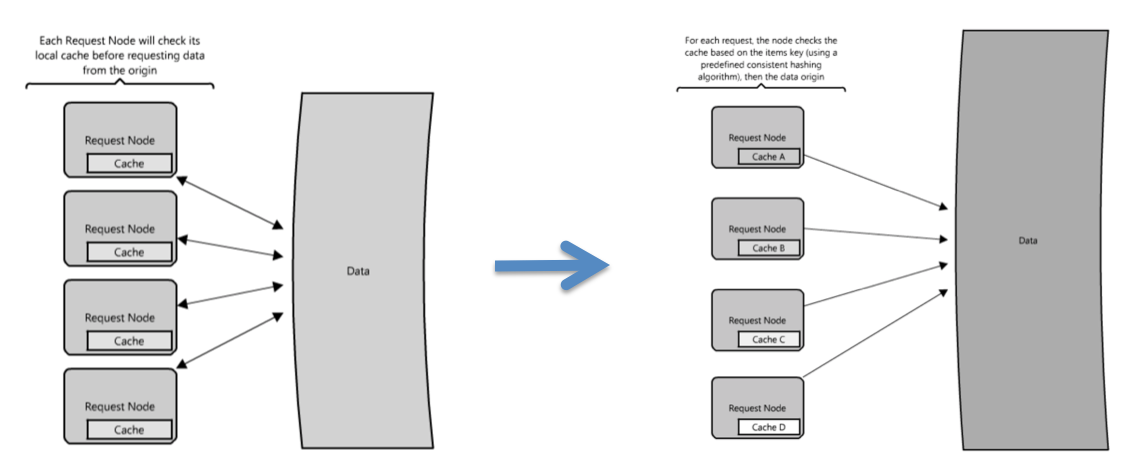
\includegraphics[width=150mm]{../LocalDistributedCache}
	\end{center}
	
	That change has the goal and the consequence of, respectively

    \optionA{Increasing performance and availability}
    \optionB{Increasing availability and decreasing performance}
    \optionC{Increasing performance and decreasing availability}
    \optionD{Increasing performance, scalability and availability}
    \putOptions

% Resposta: D
 \end{ClosedQuestion}
}

\newcommand{\qPerformanceTwoOne}{
  \begin{ClosedQuestion}
    Consider the change in the architecture associated with the use of caches in web services shown in the figure 
	
	\begin{center}
		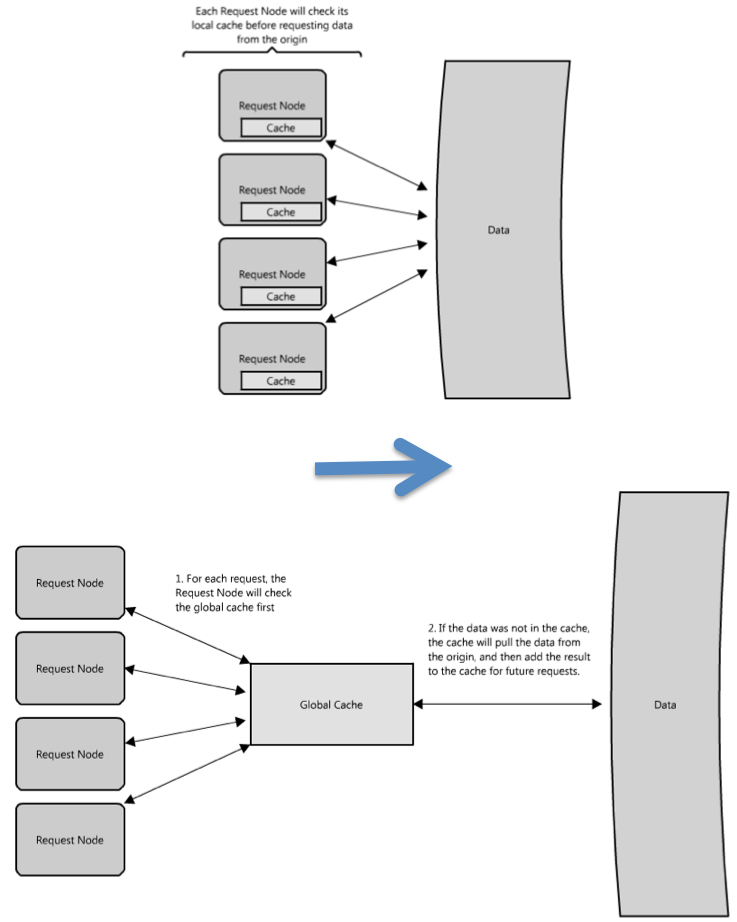
\includegraphics[width=100mm]{../LocalGlobalCache}
	\end{center}
	
	Taking into consideration that this change involves adding a server, which has a larger storage capacity than the request Nodes, that change has the impact of

    \optionA{Increasing performance and availability}
    \optionB{Increasing availability and decreasing performance}
    \optionC{Increasing performance and decreasing availability}
    \optionD{Increasing scalability and availability}
    \putOptions

% Resposta: C
  \end{ClosedQuestion}
}


%9 Modifiability
\newcommand{\qModifiabilityOneOne}{
  \begin{ClosedQuestion}
    Consider that an architect needs to design a system which interacts with two external sources of information, and it has to import some of the information to store it in the system's internal database. The stakeholders inform him that it will be necessary to include new sources of information in the future, besides the two already identified, but they cannot precisely define which they are. This changes will occur after the first version of the system is in production. Additionally, the stakeholders define a short period of time to integrate a new source of information. Given this requirements the architect should
		
    \optionA{Consider the requirements not realistic}
    \optionB{Apply tactics of defer binding to allow the addition of the new sources of information in initialization time}
    \optionC{Identify what should be the common and specific parts of the module responsible for the interaction with the external sources, before interacting again with the stakeholders}
    \optionD{Consider this requirement as a non architecturally significant requirement}

    \putOptions

% Resposta: D
 \end{ClosedQuestion}
}

\newcommand{\qModifiabilityTwoOne}{
  \begin{ClosedQuestion}
    Several of the cases studied in this course had scalability
    requirements.  That means that those systems should be designed in
    such a way that they

    \optionA{Have high throughput}
    \optionB{Have low latency}
    \optionC{Allow many simultaneous users}
    \optionD{May be easily changed to increase their performance}

    \putOptions

% Resposta: D
 \end{ClosedQuestion}
}


%10 nginx Scenarios and Tactics
\newcommand{\qNginxScenariosTacticsOne}{
\begin{ClosedQuestion}
	Consider the following excerpt from Nginx case study

	\begin{quote}
		nginx configuration is kept in a number of plain text files which typically reside in /usr/local/etc/nginx or /etc/nginx. The main configuration file is usually called nginx.conf. 		To keep it uncluttered, parts of the configuration can be put in separate files which can be automatically included in the main one. However, it should be noted here that nginx 		does not currently support Apache-style distributed configurations (i.e., .htaccess files). All of the configuration relevant to nginx web server behavior should reside in a 		centralized set of configuration files.
	\end{quote}
	
	When comparing the configuration in Nginx with the configuration in Apache we can say that
	
	  \optionA{Due to its configuration strategy Apache has better performance}
	  \optionB{Performance was the main concern of the design of the configuration strategy in Nginx}
	  \optionC{Apache emphasizes the usability quality for system administrators by allowing to split the configuration by different files}
	  \optionD{Nginx emphasizes the usability quality for system administrators by reducing the number or errors}
  
	  \putOptions
	\end{ClosedQuestion}
	}

\newcommand{\qNginxScenariosTacticsTwo}{
\begin{ClosedQuestion}
  Web servers typically receive requests from different users
  concurrently (that is, either different users make requests
  simultaneously or they make them fast enough that it is not possible
  for the web server to answer one request from one user before
  receiving another request from another user).  To process all the
  requests, web servers may use different implementation strategies.
  Assuming that we want to develop a web server to serve only static
  pages with more or less the same size to a set of clients on the
  same LAN network as the server, which of the following strategies
  would be better?

  \optionA{Launch a new process for processing each request}
  \optionB{Spawn a new thread for processing each request}
  \optionC{Put the requests into a queue and schedule their processing}
  \optionD{Buy a server with high processing power}
  
  \putOptions
\end{ClosedQuestion}
}

%11 Continuous Integration Scenarios and Tactics - NEW
\newcommand{\qContinousIntegrationScenariosTacticsOne}{
  \begin{ClosedQuestion}
	  In the Continous integration case study can be read about Jenkins
	  
	  \begin{quote}
		  It takes advantage of the JUnit XML standard for unit test and code coverage reporting to integrate reports from a variety of test tools. Jenkins originated with Sun, but is very widely used and has a robust open-source community associated with it.
	  \end{quote}
	  
	  Consider that a scenario is written from the above sentence
    
    \optionA{The stimulus is to integrate reports from a variety of test tools}
    \optionB{The response is JUnit XML standard}
    \optionC{The source of the stimulus is Sun}
    \optionD{The measure of the response is a robust open-source community associated with it}
    \putOptions

 \end{ClosedQuestion}
}

\newcommand{\qContinousIntegrationScenariosTacticsTwo}{
  \begin{ClosedQuestion}
	  In the Continous integration case study can be read about Jenkins
	  
	  \begin{quote}
		  It takes advantage of the JUnit XML standard for unit test and code coverage reporting to integrate reports from a variety of test tools. Jenkins originated with Sun, but is very widely used and has a robust open-source community associated with it.
	  \end{quote}
	  
	  The quality of Jenkins that is emphasized in the above sentence is
    
    \optionA{Modifiability}
    \optionB{Availability}
    \optionC{Testability}
    \optionD{Interoperability}
    \putOptions

 \end{ClosedQuestion}
}


%12 Infinispan Scenarios and Tactics - NEW
\newcommand{\qInfinispanScenariosTacticsOne}{
  \begin{ClosedQuestion}
	  In the Infinispan case study can be read
	  
	  \begin{quote}
		  When persisting for durability, persistence can either be online, where the application thread is blocked until data is safely written to disk, or offline, where data is flushed to disk periodically and asynchronously. In the latter case, the application thread is not blocked on the process of persistence, in exchange for uncertainty as to whether the data was successfully persisted to disk at all.
	  \end{quote}
	  
	  From the description we can infer a trade-off between the qualities of
    
    \optionA{Modifiability and Performance}
    \optionB{Availability and Modifiability}
    \optionC{Performance and Reliability}
    \optionD{Reliability and Security}
    \putOptions

 \end{ClosedQuestion}
}

\newcommand{\qInfinispanScenariosTacticsTwo}{
  \begin{ClosedQuestion}
	  In the Infinispan case study can be read
	  
	  \begin{quote}
		  Infinispan supports several pluggable cache stores-adapters that can be used to persist data to disk or any form of secondary storage. The current default implementation is a simplistic hash bucket and linked list implementation, where each hash bucket is represented by a file on the filesystem. While easy to use and configure, this isn't the best-performing implementation.
	  \end{quote}
	  
	  The main architectural quality addressed in the above excerpt is 
	  
    \optionA{Performance}
    \optionB{Modifiability}
    \optionC{Usability}
    \optionD{Security}
    \putOptions

 \end{ClosedQuestion}
}


%13 Designing-an-Architecture
\newcommand{\qDesigningArchitectureOne}{
  \begin{ClosedQuestion}
    According to the attribute-driven design process, we should design
    the software architecture for a system based on a selected list of
    requirements, which are called the \textit{architecture significant requirements}.
    These requirements should be sorted according to their
    importance for the system's stakeholders because

    \optionA{We should always satisfy in the first place the requirements
      of more important stakeholders (such as the client)}
    \optionB{If no order was established among them, we would not know
      from where should we start the design process}
    \optionC{If one of the stakeholders complains that his requirement
      is not satisfied, we may explain to him that there were other more
      important requirements first}
    \optionD{When it is not possible to satisfy all of the requirements
      optimally, we should be aware of their relative importance so that
      we may find a solution that corresponds to a satisfactory trade-off}
    \putOptions

% Resposta: D
 \end{ClosedQuestion}
}

\newcommand{\qDesigningArchitectureTwo}{
\begin{ClosedQuestion}
	During the different steps on how to create an architecture, the precise specification of architecture quality attributes is initially relevant to

    \optionA{Make a business case for the system}
    \optionB{Understand the architecturally significant requirements}
    \optionC{The system design}
    \optionD{Documenting and communicating the architecture}
 \putOptions
\end{ClosedQuestion}
}


%14 Module Viewtype
\newcommand{\qModuleViewtypeOneOne}{
  \begin{ClosedQuestion}
    Consider the following description of \emph{Memcached}, which is
    adapted from its Wiki:
    \begin{quote}
      Memcached is an in-memory key-value store for small chunks of
      arbitrary data from results of database calls, API calls, or
      page rendering.  It is made up of:
      \begin{itemize}
      \item Client software, which is given a list of available memcached servers.
      \item A client-based hashing algorithm, which chooses a server
        based on the "key" input.
      \item Server software, which stores your values with their keys
        into an internal hash table.
      \item Server algorithms, which determine when to throw out old
        data (if out of memory), or reuse memory.
      \end{itemize}
    \end{quote}
    Suppose that you want to present an architectural view for
    \emph{Memcached} that represents the above information.  Which
    view is more adequate?

    \optionA{A view of the Data Model style}
    \optionB{A view of the Layers style}
    \optionC{A view of the Decomposition style}
    \optionD{A view of the Uses style}
    \putOptions

% Resposta: C
  \end{ClosedQuestion}
}

\newcommand{\qModuleViewtypeTwoOne}{
  \begin{ClosedQuestion}
	  Suppose that in the development of an enterprise application (which needs to access a
	  database) it was decided to use the Hibernate framework to simplify the development
	  of the data access code. Which architectural view is the most adequate to represent this
	  decision?
	  
	  \optionA{A Deployment view}
	  \optionB{A Component-and-Connector view}
	  \optionC{A Uses view}
	  \optionD{A Decomposition view}
    \putOptions

% Resposta: D
  \end{ClosedQuestion}
}


%15 Uses and Generalization architectural styles
\newcommand{\qUsesGeneralizationOne}{
\begin{ClosedQuestion}
  To achieve a faster time-to-market, software companies are
  increasingly using a strategy of incremental releases of their
  software, where each new release has a set of new features.  Which
  architectural style is better to analyse whether the system's
  software architecture is adequate for the planned incremental
  releases?

  \optionA{The Decomposition style}
  \optionB{The Deployment style}
  \optionC{The Uses style}
  \optionD{The Work-assignment style}
  \putOptions
\end{ClosedQuestion}
}

\newcommand{\qUsesGeneralizationTwo}{
\begin{ClosedQuestion}
	Suppose that in the process of designing a system's software architecture you come to
	the conclusion that there are uses relations in both directions in almost all of the system's
	modules. This means that
	
	\optionA{There is a high level of communication between the several modules, and this
		will cause the system to have a low performance}
	\optionB{It is not possible to install the system in more than one machine}
	\optionC{It is not possible to develop and to test the system incrementally}
	\optionD{It is very hard to explain what the system does, because we need to understand
		all the execution fluxes}
		
  \putOptions
\end{ClosedQuestion}
}


%16 Layered, Aspects and Data Model
\newcommand{\qLayeredAspectsDataModelOne}{
\begin{ClosedQuestion}
  In a layered architecture composed by four layers, where the topmost
  layer is the layer number 1 and the bottommost layer is the layer
  number 4, which of the layers is more modifiable?

    \optionA{Layer 1}
    \optionB{Layer 4}
    \optionC{In a layered architecture all layers are equally modifiable}
    \optionD{Modifiability is not made easier by a layered architecture}
  \putOptions
\end{ClosedQuestion}
}

\newcommand{\qLayeredAspectsDataModelTwo}{
\begin{ClosedQuestion}
	 Suppose that you are implementing a module in a system that has a two layered architecture.
	 Knowing that your module belongs to the upper layer (assuming the usual notation
	 for the layer style), this means that you
	 
	 \optionA{Can use the operations defined in any of the system's modules}
	 \optionB{Can use the operations defined in the lower layer, but not the ones defined in
	 	the upper layer}
	 \optionC{Can use the operations defined in the upper layer, but not the ones defined in
	 	the lower layer}
	 \optionD{Should use some operation defined in the lower layer}
  \putOptions
\end{ClosedQuestion}
}


%17 Component and Connector
\newcommand{\qComponentConnectorOne}{
\begin{ClosedQuestion}
  Suppose that there are certain performance requirements for a
  system, and that you want to show to the stakeholders of the system
  that the software architecture that you designed meet those
  requirements. To do this

    \optionA{It makes no sense to use views of the module viewtype, as
    	they give only a static view of the system}
    \optionB{You should use only views of the component-and-connector
    	viewtype, which describe the dynamic aspects of the system}
    \optionC{You may need to use views of the three viewtypes}
    \optionD{The only views that are relevant to performance
    	requirements are views of the Deployment style}
	 
	\putOptions
\end{ClosedQuestion}
}

\newcommand{\qComponentConnectorTwo}{
\begin{ClosedQuestion}
	The connectors on component-and-connector view
	
	\optionA{Represent the network infrastructure that allows components to communicate
		with each other}
	\optionB{May, on another view of the system, be represented by a set of components
		and connectors}
	\optionC{Represent the dependency relations that exist among the various components}
	\optionD{Represent the control flow during a execution of the system}
	
	\putOptions
\end{ClosedQuestion}
}


%18 Repository and Client-Server
\newcommand{\qRepositoryClientServerOne}{
  \begin{ClosedQuestion}
    Suppose that you are designing the software architecture for an
    enterprise application that has requirements about the maximum
    response time for a certain type of requests.  Moreover, assume
    that those requests arrive at the system periodically, whereas the
    remaining requests have an unpredictable frequency.  Finally,
    assume that your system will have a single server that will be
    executing on a predefined machine with a 12-core AMD processor.
    To show to the stakeholders that your system satisfies the
    performance requirements you have to use views of which
    architectural style?

    \optionA{The Work Assignment style}
    \optionB{The Client-Server style}
    \optionC{The Deployment style}
    \optionD{The Communicating Processes style}
    \putOptions

% Resposta: D
  \end{ClosedQuestion}
}

\newcommand{\qRepositoryClientServerTwo}{
  \begin{ClosedQuestion}
    The email system is composed of various types of components
    playing different roles.  For example, to send an email, a user
    uses a \emph{mail user agent} (MUA), to compose his message and
    send it.  To send the message, the MUA typically connects to a
    \emph{mail transfer agent} (MTA) that receives the message,
    analyzes the message's headers to determine the recipients and,
    after querying the DNS system to determine the MTA responsible for
    each recipient, it connects to the MTAs responsible for the
    destination addresses to deliver the message.  Each of these MTAs
    receives the message and stores it locally or forwards it to
    others MTAs until the message reaches its destination MTA.
    The recipient user of the message will then use his MUA to see the
    messages that were sent to him.  To do it, the MUA connects to an
    IMAP or POP server to obtain the user's messages.  Those IMAP and
    POP servers obtain the messages for a user by reading the messages
    stored by the MTA.

    Given this simplified description of the operation of the email
    system, which of the following architectural styles is more
    appropriate to represent the pattern of interaction between the
    MTA and the servers IMAP and POP?

    \optionA{The Peer-to-Peer style}
    \optionB{The Client-Server style}
    \optionC{The Shared-Data style}
    \optionD{The Publish-subscribe style}

    \putOptions
  \end{ClosedQuestion}
}


%19 Tiers, Dynamic reconfiguration, Peer-to-peer, Publish-subscribe
\newcommand{\qTiersDynamicreconfigurationPeertopeerPublishsubscribeOne}{
  \begin{ClosedQuestion}
	  Typically, Instant Messaging clients have a window to list the contacts of the user, and
	  show in that window the status of each contact (whether it is available, unavailable, busy,
	  etc). Given that the status of a contact may be changed at any time, and that the contact's
	  status is given by the Instant Messaging application of that contact, which architectural
	  style represents best the interaction pattern between these components?

	   \optionA{The Shared Data style}
	   \optionB{The Pipes-and-filters style}
	    \optionC{The Publish-subscribe style}
	 \optionD{The Client-Server style}
   \putOptions

  \end{ClosedQuestion}
}

\newcommand{\qTiersDynamicreconfigurationPeertopeerPublishsubscribeTwo}{
  \begin{ClosedQuestion}
    Consider the following excerpt from the tutorial on the Hadoop
    MapReduce:

    \begin{quote}
      Hadoop MapReduce is a software framework for easily writing
      applications which process vast amounts of data (multi-terabyte
      data-sets) in-parallel on large clusters (thousands of nodes) of
      commodity hardware in a reliable, fault-tolerant manner.

      A MapReduce job usually splits the input data-set into
      independent chunks which are processed by the map tasks in a
      completely parallel manner.  The framework sorts the outputs of
      the maps, which are then input to the reduce tasks. Typically
      both the input and the output of the job are stored in a
      file-system.  The framework takes care of scheduling tasks,
      monitoring them and re-executes the failed tasks.
    \end{quote}

    Which architectural style of the component-and-connector viewtype
    is more adequate to describe how the MapReduce works, taking into
    account its main advantages in solving a problem?

    \optionA{The Shared data style}
    \optionB{The Pipes-and-filters style}
    \optionC{The Peer-to-Peer style}
    \optionD{The Communicating Processes style}
   \putOptions

% Resposta: D
  \end{ClosedQuestion}
}


%20 SOA, Pipes-and-Filters
\newcommand{\qSOAPipesFiltersOne}{
  \begin{ClosedQuestion}
	  Imagine that you want to develop a system that is to be used in email servers, whose goal
	  is to allow changing the emails that are received by the server (for example, to remove
	  potential viruses or URLs linking to phishing sites). The goal is that the server feeds each
	  received email through this system before processing it (e.g., forward it to another server,
	  or store it locally). The system is supposed to be easily modifiable, to support new types
	  of email transformations. Which architectural style is the most adequate to satisfy these
	  requirements?

	   \optionA{The Peer-to-Peer style}
	   \optionB{The Pipes-and-filters style}
	   \optionC{The Client-Server style}
	   \optionD{The Publish-subscribe style}
    \putOptions

% Resposta: B
 \end{ClosedQuestion}
}


\newcommand{\qSOAPipesFiltersTwo}{
  \begin{ClosedQuestion}
    Suppose that you are developing the software architecture of a new
    system for an organization composed of several organizational
    units, each one with its own information systems, which have been
    developed independently of each other over the course of several
    years and depending on the particular needs of each unit.  Your
    system has the goal of integrating the various existing systems,
    providing in this way not only a unified view of how the
    organization works, but also allowing the creation of new
    processes within the organization that involve more than one unit.
    Which architectural style is better suited to design such a
    system?

    \optionA{The Decomposition style}
    \optionB{The Client-Server style}
    \optionC{The Service Oriented Architecture style}
    \optionD{The Communicating Processes style}

    \putOptions

% Resposta: C
 \end{ClosedQuestion}
}


%21 Allocation viewtype
\newcommand{\qAllocationOneOne}{
\begin{ClosedQuestion}
  The Work-assignment is an architectural style of the allocation
  viewtype, where

    \optionA{Components are allocated to persons and teams}
    \optionB{Modules are allocated to persons and teams}
    \optionC{Components and modules are allocated to persons and teams}
    \optionD{None of the above}
    \putOptions

% Resposta: B
 \end{ClosedQuestion}
}

\newcommand{\qAllocationTwoOne}{
\begin{ClosedQuestion}
  In the software architecture of a system, the Deployment view is
  best suited for

    \optionA{Analysing the performance of the system}
    \optionB{Planning incremental releases of the system}
    \optionC{Estimating the effort needed to implement the system}
    \optionD{Analysing the system's portability and reusability}
    \putOptions

% Resposta: A
 \end{ClosedQuestion}
}


%22 nginx views
\newcommand{\qnginxOne}{
\begin{ClosedQuestion}
  Web servers implemented in Java, such as the Tomcat web server,
  typically use a thread-based model for processing requests.  That
  is, they process each request on a different thread within the same
  JVM process, rather than on a different process.  One of the reasons
  for this is that

  \optionA{Launching a new process for processing each request is too expensive}
  \optionB{Using threads ensures that the processing of each request is
  	isolated from the remaining requests}
  \optionC{With this approach they may use all of the available cores
  	in multiprocessor machines}
  \optionD{They are used for implementing enterprise applications that
  	typically have complex domain logic and, by using threads, it is
  	easier to reuse code from one request to another}
  \putOptions
  
  % Resposta: A
\end{ClosedQuestion}
}

\newcommand{\qnginxTwo}{
  \begin{ClosedQuestion}
    In Nginx, given that a \emph{worker} processes various requests during its
    life, how does it do it?

    \optionA{By interleaving the various processing phases of each
      request in a sequential process}
    \optionB{By executing in parallel each of the phases of the
      pipeline corresponding to the processing of a request}
    \optionC{By executing in parallel the processing of the various requests}
    \optionD{By processing completely each request before moving to
      the next one, in a sequential process}
    \putOptions
	
    % Resposta: A
  \end{ClosedQuestion}
}


%23 Continuous Integration Views - NEW
\newcommand{\qContinousIntegrationViewsOne}{
  \begin{ClosedQuestion}
	 Consider the following architectural view of the Pony-Build system as described in the Continous integration case study
	  
	\begin{center}
		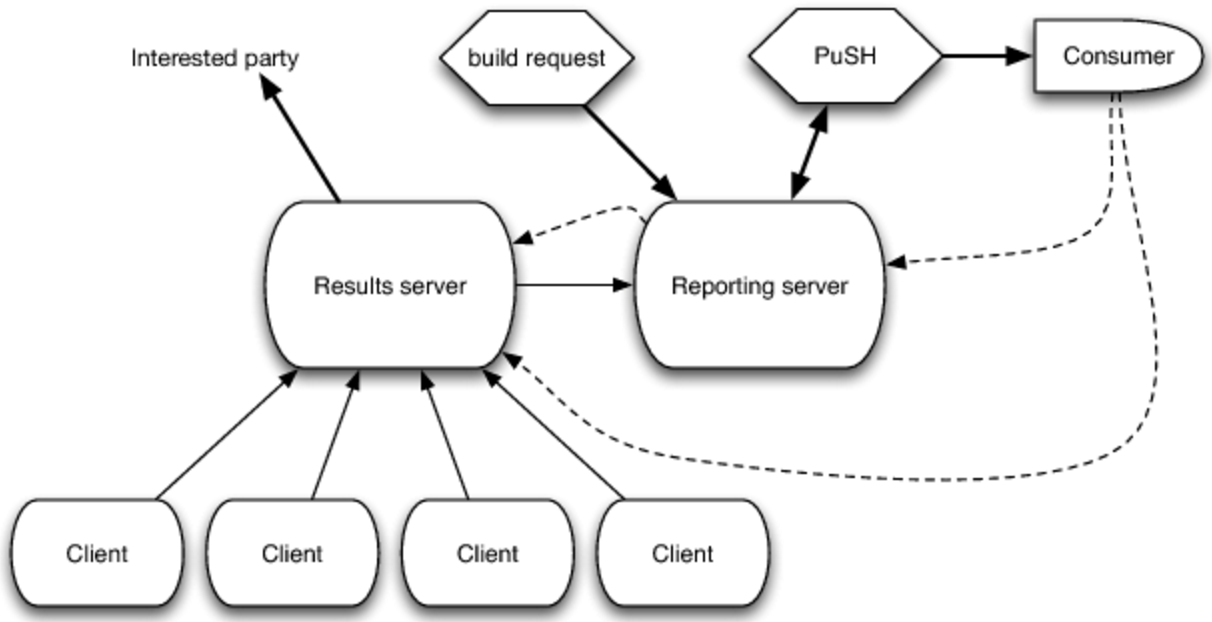
\includegraphics[width=100mm]{../PonyBuildArchitecture}
	\end{center}
	
	According to this view the quality of performance is achieved through
    
    \optionA{An increase resource efficiency tactic}
    \optionB{A schedule resources tactic}
    \optionC{A multiple copies of computation tactic}
    \optionD{A manage sampling rate tactic}
    \putOptions

 \end{ClosedQuestion}
}

\newcommand{\qContinousIntegrationViewsTwo}{
  \begin{ClosedQuestion}
	  In the Continous integration case study can be read about future features for Pony-Build
	  
	  \begin{quote}
		  Currently, each continuous integration system reinvents the wheel by providing its own build configuration language, which is manifestly ridiculous; there are fewer than a dozen commonly used build systems, and probably only a few dozen test runners. Nonetheless, each CI system has a new and different way of specifying the build and test commands to be run. In fact, this seems to be one of the reasons why so many basically identical CI systems exist: each language and community implements their own configuration system, tailored to their own build and test systems, and then layers on the same set of features above that system. Therefore, building a domain-specific language (DSL) capable of representing the options used by the few dozen commonly used build and test tool chains would go a long way toward simplifying the CI landscape.
	  \end{quote}
	  
	  Suppose that you are the architect that has to change the architecture to accomodate this new feature. Therefore, as an architect
    
    \optionA{You need to change the decomposition view to represent modules with the responsibilities associated with the DSL}
    \optionB{You need to design a client-server view representing the interaction between the DSL and the servers that execute its commands}
    \optionC{You need to design an implementation view to allow system administrators configure the builds}
    \optionD{You do not need to change the views because the DSL does not have any architectural impact}
    \putOptions

 \end{ClosedQuestion}
}


%24 Infinispan Views - NEW
\newcommand{\qInfinispanViewsOne}{
  \begin{ClosedQuestion}
	  In the Infinispan case study can be read
	  
	  \begin{quote}
		 Infinispan's core data structures make use of software transactional memory techniques for concurrent access to shared data. This minimizes the need for explicit locks, mutexes and other forms of synchronization, preferring techniques like compare-and-set operations within a loop to achieve correctness when updating shared data structures. Such techniques have been proven to improve CPU utilization in multi-core and SMP systems, and despite the increased code complexity, has paid off in overall performance when under load.
	  \end{quote}
	  
	  These properties of Infinispan can be represented by
    
    \optionA{A decomposition view which represent the module for compare-and-set}
    \optionB{A client-server view with non-blocking connectors for the interaction between threads and core data structures}
    \optionC{A communicating-processes view with non-blocking connectors for the interaction between threads and core data structures}
    \optionD{A deployment view which allocate threads to the multi-cores}
    \putOptions

 \end{ClosedQuestion}
}

\newcommand{\qInfinispanViewsTwo}{
  \begin{ClosedQuestion}
	  In the Infinispan case study can be read
	  
	  \begin{quote}
		 Infinispan uses its own serialization scheme, where full class definitions are not written to the stream. Instead, magic numbers are used for known types where each known type is represented by a single byte. This greatly improves not just serialization and de-serialization speed qualities, but also produces a much more compact byte stream for transmission across a network. An externalizer is registered for each known data type, registered against a magic number. This externalizer contains the logic to convert object to bytes and vice versa.
	  \end{quote}
	  
	  These properties of Infinispan can be represented by
    
    \optionA{A uses view which represent modules for the externalizers}
    \optionB{A client-server view which represent the byte stream for transmission across a network}
    \optionC{A connector that has the serialization and de-serialization speed qualities}
    \optionD{A decomposition view which contains the serialization/de-serilization modules}
    \putOptions

 \end{ClosedQuestion}
}


%25 Web2.0 
\newcommand{\qWebTwoOne}{
  \begin{ClosedQuestion}
    With the evolution of the web application technologies, it is now
    possible to develop web applications with a user interface similar
    to the interface of desktop applications.  Yet, for this to
    happen, part of the code that was executing in the web server is
    now executing in the web browser.  How does this change manifests
    in the software architecture of the system?

    \optionA{In the Deployment view, because the presentation
      component is now executing in a different place}
    \optionB{In the component-and-connector view, because the
      connector between the web client and the web server has to change}
    \optionC{In the Layer view, because the order of the layers will
      have to change}
    \optionD{In the mapping between layers of the system and the
      components where they execute}
    \putOptions

% Resposta: D
  \end{ClosedQuestion}
}

\newcommand{\qWebTwoTwo}{
  \begin{ClosedQuestion}
    One of the evolutions in the development of web applications was
    the appearance of \emph{mashups}, which are described in Wikipedia
    as follows:

    \begin{quote}
      In web development, a mashup is a web page or application that
      uses and combines data, presentation or functionality from two
      or more sources to create new services.
    \end{quote}

    Knowing that the sources used by \emph{mashups} do not know about
    the existence of the \emph{mashups} and that they change
    frequently, forcing the adaptation of the \emph{mashups} to
    accomodate those changes, what is the best architecture to
    minimize the effects of those changes?

    \optionA{A \emph{web services} architecture}
    \optionB{A Client-Server architecture, where the \emph{mashup}
      is the client and the various sources are the servers}
    \optionC{A layered architecture, where the access to the various
      sources is the responsibility of the bottommost layer}
    \optionD{A Publish-Subscribe architecture, where the various
      sources publish events with the changes made and the
      \emph{mashup} subscribes those events}
    \putOptions

% Resposta: C
  \end{ClosedQuestion}
}


%26 Microservices architecture - NEW
\newcommand{\qMicroservicesArchitectureOne}{
  \begin{ClosedQuestion}
    Consider the following figure depicting two different architectures for web applications
	
	\begin{center}
		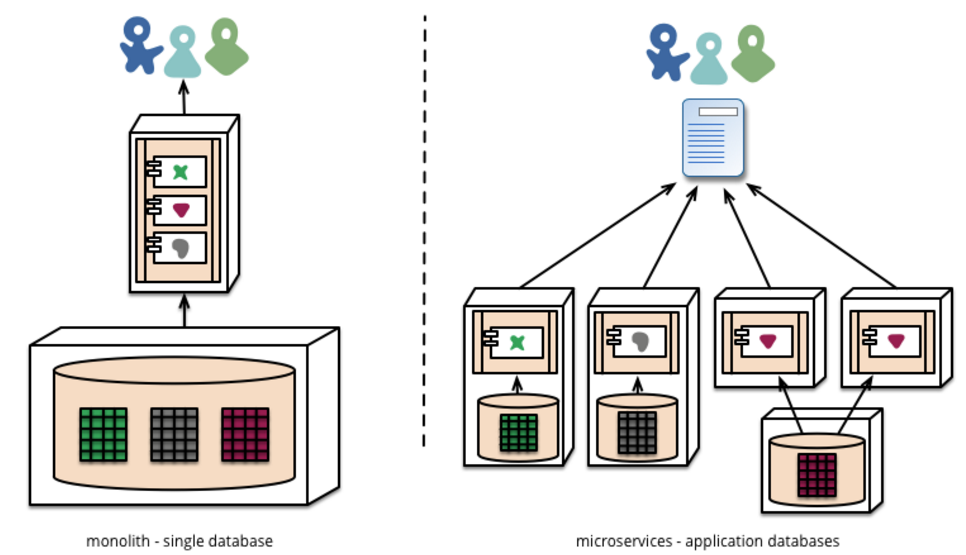
\includegraphics[width=100mm]{../Microservices}
	\end{center}
	
    \optionA{The left part of the figure represents a three-layered architecture}
    \optionB{The most relevant architectural style in the right part of the figure is shared-data}
    \optionC{The system represented in the left part of the figure tends to be non-transactional}
    \optionD{The system represented in the right part of the figure tends to have good modifiability}
    \putOptions

 \end{ClosedQuestion}
}

\newcommand{\qMicroservicesArchitectureTwo}{
  \begin{ClosedQuestion}
    Consider the following figure depicting two different architectures for web applications
	
	\begin{center}
		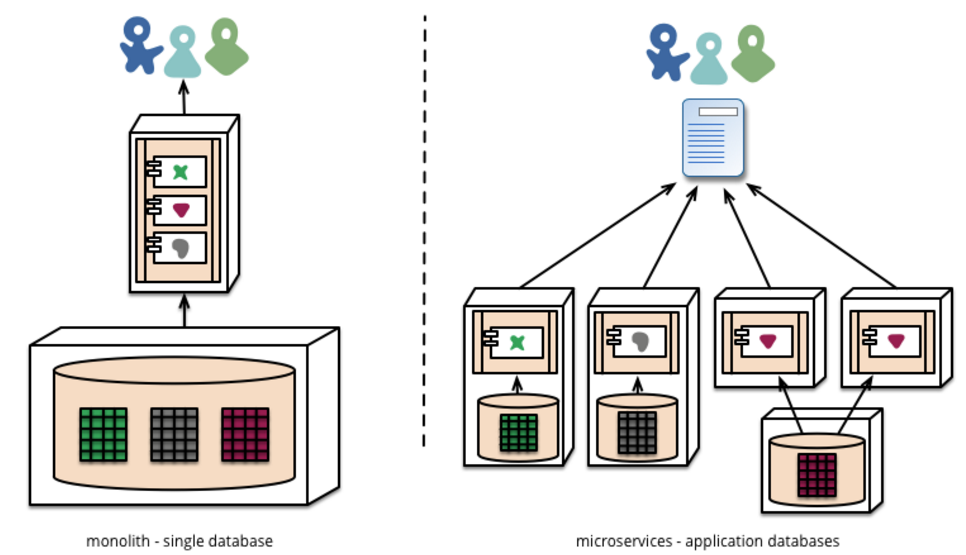
\includegraphics[width=140mm]{../Microservices}
	\end{center}
	
    \optionA{The main quality of the system in the right part of the figure is scalability}
    \optionB{The main quality of the system in the left part of the figure is scalability}
    \optionC{The main quality of the system in the right part of the figure is ease of development}
    \optionD{The main quality of the system in the left part of the figure is to promote cross-functional teams}
    \putOptions

 \end{ClosedQuestion}
}


%27 Amazon - NEW
\newcommand{\qAmazonOne}{
  \begin{ClosedQuestion}
    Consider the following excerpt about the Amazon system
	
	\begin{quote}
		Over time, this grew into hundreds of services and a number of application servers that aggregate the information from the services. The application that renders the Amazon.com Web pages is one such application server, but so are the applications that serve the Web-services interface, the customer service application, the seller interface, and the many third-party Web sites that run on our platform.
	\end{quote}
	
	The architectural style that better represents these aspects of the Amazon architecture is
	
    \optionA{Service-oriented architecture to express how clients can access the services}
    \optionB{Client-server to express how multiple clients can access the applications}
    \optionC{Tiers to express that different applications define their own contexts}
    \optionD{Decomposition to express the different responsibilities assigned to each application}
    \putOptions

 \end{ClosedQuestion}
}

\newcommand{\qAmazonTwo}{
  \begin{ClosedQuestion}
    Consider the following excerpt about the Amazon system
	
	\begin{quote}
		Mainly, I think service orientation has helped us there. The stored data formats are decoupled from the format in which you communicate data items. If there is no need for sharing schemas of the actual storage layout, you can focus on making sure that the service interfaces can evolve in a way that allows you to handle variations of data formats. You could dictate a rigorous single format, but that would not be realistic if you are in Amazon's platform business. We have to make sure that the platform can be extended by our customers to meet their needs.
	\end{quote}
	
	The architectural style that better represents these aspects of the Amazon architecture is
	
    \optionA{Data model to express the stored data formats}
    \optionB{Decomposition to express the services interfaces}
    \optionC{Aspects to express the evolution of service interfaces}
    \optionD{Publish-subscribe to express how data is shared between services}
    \putOptions

 \end{ClosedQuestion}
}


%28 Scalable web architecture and distributed systems tactics - NEW
\newcommand{\qScalableArchitectureOne}{
  \begin{ClosedQuestion}
    Consider the following excerpt about the Scalable web architecture and distributed systems case study about two different possible implementations of a global cache
	
	\begin{quote}
		 The majority of applications leveraging global caches tend to use the first type, where the cache itself manages eviction and fetching data to prevent a flood of requests for the same data from the clients. However, there are some cases where the second implementation makes more sense. For example, if the cache is being used for very large files, a low cache hit percentage would cause the cache buffer to become overwhelmed with cache misses; in this situation it helps to have a large percentage of the total data set (or hot data set) in the cache. 	\end{quote}
	
    \optionA{The solution where the application is responsible for the eviction has better availability}
    \optionB{The solution where the cache is responsible for the eviction has better availability}
    \optionC{The solution where the application is responsible for the eviction has better modifiability}
    \optionD{The solution where the cache is responsible for the eviction has better performance}
    \putOptions

 \end{ClosedQuestion}
}

\newcommand{\qScalableArchitectureTwo}{
  \begin{ClosedQuestion}
    Consider the following excerpt about the Scalable web architecture and distributed systems case study
	
	\begin{quote}
		 Employing such a strategy maximizes data locality for the requests, which can result in decreased request latency. For example, let's say a bunch of nodes request parts of B: partB1, partB2, etc. We can set up our proxy to recognize the spatial locality of the individual requests, collapsing them into a single request and returning only bigB, greatly minimizing the reads from the data origin.
	\end{quote}
	
	The quality that is achieved with this tactic is
	
    \optionA{Performance because all requests will be processed faster}
    \optionB{Performance because it allows the processing of more requests per unit of time}
    \optionC{Availability because even if PartB1 is not available partB2 can be provided}
    \optionD{Reliability because a single correct read is used to responde to several requests}
    \putOptions

 \end{ClosedQuestion}
}


%29 Graphite scenarios and tactics
\newcommand{\qGraphiteScenarioTacticsOne}{
  \begin{ClosedQuestion}
    In the Graphite system the component \emph{carbon} provides to \emph{webapp} components an access interface to the \emph{buffers} in order to improve the quality of

    \optionA{Performance}
    \optionB{Interoperability}
    \optionC{Reliability}
    \optionD{Security}

     \putOptions
% Resposta: C
   \end{ClosedQuestion}
}

\newcommand{\qGraphiteScenarioTacticsTwo}{
  \begin{ClosedQuestion}
	  Which quality, or qualities, of the Graphite system are described by the sentence: \emph{Graphite's Composer UI provides a point-and-click method to create a graph from which you can simply copy and paste the URL.}

    \optionA{Usability and Performance}
    \optionB{Usability}
    \optionC{Performance}
    \optionD{Testability}

     \putOptions
% Resposta: B
   \end{ClosedQuestion}
}


% 30 Graphite views
\newcommand{\qGraphiteViewsOne}{
 \begin{ClosedQuestion}
    In Graphite system  the \emph{receiver} and the \emph{writer threads} support asynchronous writing of metrics to optimize disk accesses. The interaction between these two components follow the architectural style

    \optionA{Client-server}
    \optionB{Communicating Processes}
    \optionC{Repository}
    \optionD{Pipes-and-Filters}

     \putOptions
% Resposta: B
   \end{ClosedQuestion}
}

\newcommand{\qGraphiteViewsTwo}{
  \begin{ClosedQuestion}
	  A high-level component-and-connect view of Graphite system can be designed using only the architectural style(s)

    \optionA{Shared-data and Communicating-Processes}
    \optionB{Communicating-Processes}
    \optionC{Tiers}
    \optionD{Client-Server and Shared-data}

     \putOptions
% Resposta: D
   \end{ClosedQuestion}
}